\section{Physic Object Recostruction}

\subsection{Primary Vertices object definition}

\begin{table}[htb]
	\caption{definition of Vertex.}
	\label{table:vertexobjdefinition}
	\ttfamily\scriptsize\selectfont
	\begin{center}
		\begin{tabular}{|l|ll|}
			\hline
			\multicolumn{3}{|l|}{collection \texttt{label: recoVertex}}\\
			\multicolumn{3}{|l|}{type: \texttt{offlinePrimaryVertices}}\\
			\hline
			vertex.size() & $>$ & 0 \\
			\hline
		\end{tabular}
	\end{center}
\end{table}

\subsection{Trigger Paths definition}

\begin{table}[htb]

	\caption{Trigger paths list.}
	\label{table:triggerdefinition}
	\ttfamily\scriptsize\selectfont
	\begin{center}
		\begin{tabular}{|l|l|}
			\hline
			\multicolumn{2}{|l|}{collection \texttt{label: TriggerResults\_HLT}}\\
			\multicolumn{2}{|l|}{type: \texttt{edm::TriggerResults}}\\
			\hline
			\texttt{HLT\_DoubleMediumIsoPFTau35\_Trk5\_eta2p1\_Prong1\_v2} & OR \\
			\texttt{HLT\_DoubleMediumIsoPFTau35\_Trk5\_eta2p1\_Prong1\_v3} & OR \\
			\texttt{HLT\_DoubleMediumIsoPFTau35\_Trk5\_eta2p1\_Prong1\_v4} & OR \\
			\texttt{HLT\_DoubleMediumIsoPFTau35\_Trk5\_eta2p1\_Prong1\_v6} & OR \\
			\texttt{HLT\_DoubleMediumIsoPFTau35\_Trk1\_eta2p1\_Prong1\_v1} & OR \\
			\texttt{HLT\_DoubleMediumIsoPFTau35\_Trk1\_eta2p1\_Prong1\_v3} & OR \\
			\texttt{HLT\_DoubleMediumIsoPFTau35\_Trk1\_eta2p1\_Prong1\_v4} & \\
			\hline
		\end{tabular}
	\end{center}
\end{table}

\clearpage

\subsection{Jet object definition}

\begin{table}[htb]
  \caption{definition of jets.}
   \label{table:jetobjdefinition}
  \begin{center}
    \ttfamily\scriptsize\selectfont
    \begin{tabular}{|l|ll|}
      \hline
      \multicolumn{3}{|l|}{ collection label: selectedPatJets}\\
      \multicolumn{3}{|l|}{ type: \texttt{pat::Jet}}\\
      \hline
      jet.pt() & $>=$ & 30. \\
      fabs(jet.eta()) & $<=$ & 5.0 \\
      jet.neutralHadronEnergyFraction() & $<$ &  0.99 \\
      jet.neutralEmEnergyFraction() & $<$ & 0.99 \\
      jet.numberOfDaughters() & $>$& 1 \\
      if(fabs(jet.eta()) $<$ 2.4) && \\
      ~~~jet.chargedHadronEnergyFraction() & $>$ & 0 \\
      ~~~jet.chargedEmEnergyFraction() & $<$ & 0.99 \\
      ~~~jet.chargedMultiplicity() & $>$ & 0 \\
      DeltaR(jet,tau) & $>=$ & 0.3 \\
      \hline
    \end{tabular}
  \end{center}
\end{table}

\subsection{b-Jet object definition}

\begin{table}[htb]
  \caption{definition of $b$-jets.}
  \label{table:bjetobjdefinition}
  \begin{center}
  \ttfamily\scriptsize\selectfont
  \begin{tabular}{|l|ll|}
    \hline
    \multicolumn{3}{|l|}{ collection label: selectedPatJets}\\
    \multicolumn{3}{|l|}{ type: \texttt{pat::Jet}}\\
    \hline
    jet.pt() & $>=$ &  30. \\
    fabs(jet.eta()) & $<=$ & 2.4 \\
    DeltaR(jet,tau) & $>=$ & 0.3 \\
    jet.bDiscriminator(?) & $>$ & 0.244 \\
    \hline
  \end{tabular}
  \end{center}
\end{table}

\subsection{Tau object definition}

\begin{table}[htb]
  \caption{definition of \ensuremath{\tau} leptons.}
  \label{table:tauobjdefinition}
  \begin{center}
  \ttfamily\scriptsize\selectfont
  \begin{tabular}{|l|ll|}
    \hline
    \multicolumn{3}{|l|}{ collection label: \texttt{patTaus}}\\
    \multicolumn{3}{|l|}{ type: \texttt{pat::Tau}}\\
    \hline
    fabs(tau.eta()) & $<=$ & 2.1 \\
    tau.pt() & $>=$ & 45.0 \\
    tau.leadPFChargedHadrCand()-$>$pt() & $>=$ & 5.0 \\
    tau.tauID(``byTightIsolationMVA3newDMwLT'') & $>$ & 0.5 ||\\
    ~tau.tauID(``byMediumIsolationMVA3newDMwLT'') & $>$ & 0.5 ||\\
    ~tau.tauID(``byLooseIsolationMVA3newDMwLT'') & $>$ & 0.5 \\
    (decayModeFindingNewDMs & $>$ & 0.5 $\&\&$ \\
    ~signalPFChargedHadrCands().size() & $==$ & 1) \\
    tau.tauID(``againstElectronMediumMVA5'') & $>$ & 0.5 \\
    tau.tauID(``againstMuonLoose3'') & $>$ & 0.5 \\
    \hline
  \end{tabular}
  \end{center}
\end{table}

\clearpage

\subsection{MET object definition}

\begin{table}[htb]
  \caption{definition of \met}
  \label{table:metobjdefinition}
  \ttfamily\scriptsize\selectfont
  \begin{center}
   \begin{tabular}{|l|ll|}
      \hline
      \multicolumn{3}{|l|}{ collection \texttt{label: patMET}}\\
      \multicolumn{3}{|l|}{ type: \texttt{patPfMetT0pcT1Txy}}\\
      \hline
    \end{tabular}
  \end{center}
\end{table}

\section{Physic Object Recostruction at 13 TeV}

\subsection{Tau object definition}

\begin{table}[htb]
	\caption{definition of \ensuremath{\tau} leptons.}
	\label{table:tauobjdefinition_13TeV}
	\begin{center}
		\ttfamily\scriptsize\selectfont
		\begin{tabular}{|l|ll|}
			\hline
			\multicolumn{3}{|l|}{ collection label: \texttt{patTaus}}\\
			\multicolumn{3}{|l|}{ type: \texttt{pat::Tau}}\\
			\hline
			fabs(tau.eta()) & $<=$ & 2.1 \\
			tau.pt() & $>=$ & 20 \\
			tau.leadPFChargedHadrCand()-$>$pt() & $>=$ & 5.0 \\
			tau.tauID(``byTightIsolationMVArun2v1DBdR03oldDMwLT'') & $>$ & 0.5 ||\\
			~tau.tauID(``byMediumIsolationMVArun2v1DBdR03oldDMwLT'') & $>$ & 0.5 ||\\
			~tau.tauID(``byLooseIsolationMVArun2v1DBdR03oldDMwLT'') & $>$ & 0.5 \\
			(byLooseIsolationMVArun2v1DBnewDMwLT & $>$ & 0.5 $\&\&$ \\
			~signalPFChargedHadrCands().size() & $<$ & 4) \\
			tau.tauID(``againstElectronMediumMVA6'') & $>$ & 0.5 \\
			tau.tauID(``againstMuonLoose3'') & $>$ & 0.5 \\
			\hline
		\end{tabular}
	\end{center}
\end{table}

\subsection{Jet object definition}

\begin{table}[htb]
	\caption{definition of jets.}
	\label{table:jetobjdefinition_13TeV}
	\begin{center}
		\ttfamily\scriptsize\selectfont
		\begin{tabular}{|l|ll|}
			\hline
			\multicolumn{3}{|l|}{ collection label: selectedPatJets}\\
			\multicolumn{3}{|l|}{ type: \texttt{pat::Jet}}\\
			\hline
			jet.pt() & $>=$ & 30. \\
			fabs(jet.eta()) & $<=$ & 5.0 \\
			jet.neutralHadronEnergyFraction() & $<$ &  0.99 \\
			jet.neutralEmEnergyFraction() & $<$ & 0.99 \\
			jet.numberOfDaughters() & $>$& 1 \\
			if(fabs(jet.eta()) $<$ 2.4) && \\
			~~~jet.chargedHadronEnergyFraction() & $>$ & 0 \\
			~~~jet.chargedEmEnergyFraction() & $<$ & 0.99 \\
			~~~jet.chargedMultiplicity() & $>$ & 0 \\
			DeltaR(jet,tau) & $>=$ & 0.3 \\
			\hline
		\end{tabular}
	\end{center}
\end{table}

\section{Monte Carlo Samples at 8 TeV}
\label{sec::sampleslist_8tev}

\begin{table}[ht]
	\tiny
	\centering{
		\begin{tabular}{| l | l |}
			\hline
			&\\
			Process &Official CMS Datasets /DY*/AODSIM \\
			&\\
			\hline
			&\\
			$Z \longrightarrow \tau\tau$ & \texttt{ToTauTau\_M-20\_CT10\_TuneZ2star\_v2\_8TeV-powheg-tauola-pythia6/Summer12 DR53X-PU\_S10\_START53\_V7A-v2} \\
			&\\
			$Z \longrightarrow \mu\mu$ & \texttt{ToMuMu\_M-20\_CT10\_TuneZ2star\_v2\_8TeV-powheg-pythia6/Summer12\_DR53X-PU\_S10\_START53\_V7A-v1} \\
			&\\
			$Z \longrightarrow ee$ & \texttt{ToEE\_M-20\_CT10\_TuneZ2star\_v2 8TeV-powheg-pythia6/Summer12\_DR53X-PU\_S10\_START53 V7A-v1} \\
			&\\
			$Z \longrightarrow ll~(10 < m_{ll} < 50)$ & \texttt{JetsToLL\_M-10To50\_TuneZ2Star\_8TeV-madgraph/Summer12\_DR53X-PU\_S10\_START53\_V7A-v1} \\
			&\\
			$Z \longrightarrow ll~(m_{ll} > 50)$ & \texttt{JetsToLL\_M-50\_TuneZ2Star\_8TeV-madgraph-tarball/Summer12\_DR53X-PU\_S10 START53\_V7A-v1} \\
			&\\
			$Z \longrightarrow ll + 1jets$ &
			\texttt{1JetsToLL\_M-50\_TuneZ2Star\_8TeV-madgraph/Summer12\_DR53X-PU\_S10 START53\_V7A-v1} \\
			&\\
			$Z \longrightarrow ll + 2jets$ & \texttt{2JetsToLL\_M-50\_TuneZ2Star\_8TeV-madgraph/Summer12\_DR53X-PU\_S10\_START53\_V7A-v1} \\
			&\\
			$Z \longrightarrow ll + 3jets$ &
			\texttt{3JetsToLL\_M-50\_TuneZ2Star\_8TeV-madgraph/Summer12 DR53X-PU\_S10\_START53\_V7A-v1} \\
			&\\
			$Z \longrightarrow ll + 4jets$ &
			\texttt{4JetsToLL\_M-50\_TuneZ2Star\_8TeV-madgraph/Summer12 DR53X-PU\_S10\_START53\_V7A-v1} \\
			&\\
			$Z \longrightarrow ll~EWK$ &
			\texttt{JJ01JetsToLL\_M-50\_MJJ-200\_TuneZ2Star 8TeV-madgraph\_tauola/Summer12\_DR53X-PU\_S10 START53\_V7A-v1} \\
			&\\
			\hline
		\end{tabular}
	}
	\caption{ Drell Yang simulated samples.}
	\label{table:samples_DY} % is used to refer this table in the text
\end{table}

\begin{table}[ht]
	\tiny
	\centering{
		\begin{tabular}{| l | l |}
			\hline
			&\\
			Process &Official CMS Datasets /W*/AODSIM \\
			&\\
			\hline
			&\\
			W + 0 jets & \texttt{JetsToLNu\_TuneZ2Star\_8TeV-madgraph-tarball/Summer12\_DR53X-PU\_S10 START53\_V7A-v2} \\
			&\\
			W + 1 jet & \texttt{1JetsToLNu\_TuneZ2Star\_8TeV-madgraph/Summer12\_DR53X-PU\_S10\_START53\_V7A-v1} \\
			&\\
			W + 2 jets & \texttt{2JetsToLNu\_TuneZ2Star\_8TeV-madgraph/Summer12\_DR53X-PU\_S10\_START53\_V7A-v1} \\
			&\\
			W + 3 jets &
			\texttt{3JetsToLNu\_TuneZ2Star\_8TeV-madgraph/Summer12\_DR53X-PU\_S10 START53\_V7A-v1} \\
			&\\
			W + 4 jets & \texttt{4JetsToLNu\_TuneZ2Star\_8TeV-madgraph/Summer12\_DR53X-PU\_S10\_START53\_V7A-v1} \\
			&\\
			\hline
		\end{tabular}
	}
	\caption{ W boson plus additional jets simulated samples.}
	\label{table:samples_Wjets} % is used to refer this table in the text
\end{table}

\begin{table}[ht]
	\tiny
	\centering{
		\begin{tabular}{| l | l |}
			\hline
			&\\
			Process &Official CMS Datasets /TTJets*/AODSIM \\
			&\\
			\hline
			\ttbar & \texttt{MassiveBinDECAY\_TuneZ2star\_8TeV-madgraph-tauola/Summer12\_DR53X-PU\_S10\_START53\_V7C-v1} \\
			&\\

			&\\
			\hline
		\end{tabular}
	}
	\caption{Standard model top production simulated sample.}
	\label{table:samples_ttbar} % is used to refer this table in the text
\end{table}

\begin{table}[ht]
	\tiny
	\centering{
		\begin{tabular}{| l | l |}
			\hline
			&\\
			Process &Official CMS Datasets */AODSIM \\
			&\\
			\hline
			&\\
			$WW(\longrightarrow 2l2\nu)$ & \texttt{WJetTo2L2Nu\_8TeV-powheg-pythia6/Summer12\_DR53X-PU\_S10\_START53\_V7C-v1} \\
			&\\
			$W^{+}W^{+}$ & \texttt{/WpWpqq\_8TeV-madgraph/Summer12\_DR53X-PU\_S10\_START53\_V7A-v1} \\
			&\\
			$W^{−}W^{−}$ & \texttt{/WmWmqq\_TeV-madgraph/Summer12\_R53X-PU\_10\_START53\_V7A-v1} \\
			&\\
			WW double scattering & \texttt{/WW\_DoubleScattering\_8TeV-pythia8/Summer12\_DR53X-PU\_S10\_START53\_V7A-v1} \\
			&\\
			WW EWK & \texttt{/WWjjTo2L2Nu\_8TeV\_madgraph\_qed6\_qcd0/Summer12\_DR53X-PU\_S10\_\_V19-v1} \\
			&\\
			$WZ~(\longrightarrow 2q2\nu)$ & \texttt{/WZJetsTo2Q2Nu\_TuneZ2star\_8TeV-madgraph-tauloa/Summer12\_DR53X-PU\_S10\_START53\_V7A-v1} \\
			&\\
			$WZ~(\longrightarrow 2l2\nu)$ & \texttt{/WZJetsTo2L2Nu\_TuneZ2star\_8TeV-madgraph-tauloa/\_DR53X-PU\_S10\_START53\_V7A-v1} \\
			&\\
			$WZ~(\longrightarrow 3l)$ & \texttt{/WZJetsTo3L\_TuneZ2star\_8TeV-madgraph-tauloa/Summer12\_DR53X-PU\_S10 START53\_V7A-v1} \\
			&\\
			$ZZ~(\longrightarrow 2q2\nu)$ & \texttt{/ZZJetsTo2Q2Nu\_TuneZ2star\_8TeV-madgraph-tauloa/Summer12\_DR53X-PU\_S10\_START53\_V7A-v1} \\
			&\\
			$ZZ~(\longrightarrow 2l2\nu)$ & \texttt{/ZZJetsTo2L2Nu\_TuneZ2star\_8TeV-madgraph-tauloa/Summer12\_DR53X-PU\_S10\_START53\_V7A-v1} \\
			&\\
			$ZZ~(\longrightarrow 2l2q)$ & \texttt{/ZZJetsTo2L2Q\_TuneZ2star\_8TeV-madgraph-tauloa/Summer12\_DR53X-PU\_S10\_START53\_V7A-v1} \\
			&\\
			$ZZ~(\longrightarrow 4l)$ & \texttt{/ZZJetsTo4L\_TuneZ2star\_8TeV-madgraph-tauloa/Summer12\_DR53X-PU\_S10\_START53\_V7A-v1} \\

			&\\
			\hline
		\end{tabular}
	}
	\caption{ Standard model production of two vector bosons simulated samples.}
	\label{table:samples_VV} % is used to refer this table in the text
\end{table}

\begin{table}[ht]
	\tiny
	\centering{
		\begin{tabular}{| l | l |}
			\hline
			&\\
			Process &Official CMS Datasets /VBF */AODSIM \\
			&\\
			\hline
			&\\
			$H \longrightarrow WW(\longrightarrow 2l)$ & \texttt{HToWWTo2LAndTau2Nu\_M-125\_8TeV-powheg-pythia6/Summer12\_DR53X-\_S10\_START53\_V7A-v1} \\
			&\\
			$H \longrightarrow ZZ(\longrightarrow 2l2\nu)$ & \texttt{HToZZTo2L2Nu\_M-120\_8TeV-powheg-pythia6/Summer12\_DR53X-PU\_S10\_START53\_V7A-v1} \\
			&\\
			$H \longrightarrow ZZ~(\longrightarrow 2l2q)$ & \texttt{HToZZTo2L2Q\_M-125\_8TeV-powheg-pythia6/Summer12\_DR53X-PU\_S10\_START53\_V7A-v1} \\
			&\\
			$H \longrightarrow ZZ~(→ 4l)$ & \texttt{HToZZTo4L\_M-125\_8TeV-powheg-pythia6/Summer12\_DR53X-PU\_S10\_START53\_V7A-v1} \\
			&\\
			$H \longrightarrow ZZ~(\longrightarrow 4\nu)$ & \texttt{HToZZTo4Nu\_M-120\_8TeV-pythia6/Summer12\_DR53X-PU\_S10\_START53\_V7A-v1} \\
			&\\
			$H \longrightarrow \tau\tau$ & \texttt{HToTauTau\_M-125\_8TeV-powheg-pythia6/Summer12\_DR53X-PU\_S} \\
			&\\
			\hline
		\end{tabular}
	}
	\caption{Standard model Higgs production by vector boson fusion simulated
		samples}
	\label{table:samples_higgs} % is used to refer this table in the text
\end{table}

\begin{table}[ht]
	\tiny
	\centering{
		\begin{tabular}{| l | l |}
			\hline
			&\\
			Process &Official CMS Datasets /VBF */AODSIM \\
			&\\
			\hline
			&\\
			$bg \longrightarrow tW^{-}$ & \texttt{/T\_tW-channel-DR\_TuneZ2star\_8TeV-powheg-tauola/Summer12\_DR53X-PU\_S10 START53\_V7A-v1} \\
			&\\
			$bg \longrightarrow tW^{+}$ & /Tbar \texttt{tW-channel-DR\_TuneZ2star\_8TeV-powheg-tauola/Summer12\_DR53X-PU\_S10\_START53\_V7A-v1} \\
			&\\
			q\textquoteright b \ensuremath{\longrightarrow} qt & \texttt{/T\_t-channel\_TuneZ2star\_8TeV-powheg-tauola/Summer12\_DR53X-PU\_S10\_START53\_V7A-v1} \\
			&\\
			$qb \longrightarrow q’t$ & \texttt{/Tbar\_t-channel\_TuneZ2star\_8TeV-powheg-tauola/Summer12\_DR53X-PU\_S10\_START53\_V7A-v1} \\
			&\\
			qq\textquoteright \ensuremath{\longrightarrow} tb & \texttt{/T\_s-channel\_TuneZ2star\_8TeV-powheg-tauola/Summer12\_DR53X-PU\_S10\_START53\_V7A-v1} \\
			&\\
			qq\textquoteright \ensuremath{\longrightarrow} tb & \texttt{/Tbar\_s-channel\_TuneZ2star\_8TeV-powheg-tauola/Summer12\_DR53X-PU\_S10\_START53\_V7A-v1} \\

			&\\
			\hline
		\end{tabular}
	}
	\caption{Single top simulated samples.}
	\label{table:samples_singlet} % is used to refer this table in the text
\end{table}

\clearpage


\section{Monte Carlo Samples at 13 TeV}
\label{sec::sampleslist_13tev}

\begin{table}[ht]
	\tiny
	\centering{
		\begin{tabular}{| l | l |}
			\hline
			&\\
			Process &Official CMS Datasets QCD*/RunIISpring15MiniAODv2 \\
			&\\
			\hline
			&\\
			QCD $100 < \HT < 200\gev$ & \texttt{HT100to200\_TuneCUETP8M1\_13TeV\-madgraphMLM\-pythia8/}	\\
			&\\
			QCD $200 < \HT < 300\gev$ & \texttt{HT200to300\_TuneCUETP8M1\_13TeV\-madgraphMLM\-pythia8/}	\\
			&\\
			QCD $300 < \HT < 500\gev$ & \texttt{HT300to500\_TuneCUETP8M1\_13TeV\-madgraphMLM\-pythia8/}	\\
			&\\
			QCD $500 < \HT < 700\gev$ & \texttt{HT500to700\_TuneCUETP8M1\_13TeV\-madgraphMLM\-pythia8/}	\\
			&\\
			QCD $700 < \HT < 1000\gev$ & \texttt{HT700to1000\_TuneCUETP8M1\_13TeV\-madgraphMLM\-pythia8/} \\
			&\\
			QCD $1000 < \HT < 1500\gev$ & \texttt{HT1000to1500\_TuneCUETP8M1\_13TeV\-madgraphMLM\-pythia8/}	\\
			&\\
			QCD $1500 < \HT < 2000\gev$ & \texttt{HT1500to2000\_TuneCUETP8M1\_13TeV\-madgraphMLM\-pythia8/}	\\
			&\\
			QCD $2000 < \HT < \infty\gev$ & \texttt{HT2000toInf\_TuneCUETP8M1\_13TeV\-madgraphMLM\-pythia8/}	\\
			&\\
			\hline
		\end{tabular}
	}
	\caption{QCD simulated samples.}
	\label{table:samples_QCD_13tev} % is used to refer this table in the text
\end{table}

\begin{table}[ht]
	\tiny
	\centering{
		\begin{tabular}{| l | l |}
			\hline
			&\\
			Process &Official CMS Datasets DYJetsToLL\_M\-50*/RunIISpring15MiniAODv2 \\
			&\\
			\hline
			&\\
			DYJetsToLL $100 < \HT < 200\gev$ & \texttt{HT\-100to200\_Tune4C\_13TeV\-madgraph\-tauola/}	\\
			&\\
			DYJetsToLL $200 < \HT < 400\gev$ & \texttt{HT\-200to400\_Tune4C\_13TeV\-madgraph\-tauola/}	\\
			&\\
			DYJetsToLL $400 < \HT < 600\gev$ & \texttt{HT\-400to600\_Tune4C\_13TeV\-madgraph\-tauola/}	\\
			&\\
			DYJetsToLL $600 < \HT < \infty\gev$ & \texttt{HT\-600toInf\_Tune4C\_13TeV\-madgraph\-tauola/}	\\
			&\\
			\\
			\hline
		\end{tabular}
	}
	\caption{Drell-Yan simulated samples.}
	\label{table:samples_DY_13tev} % is used to refer this table in the text
\end{table}

\begin{table}[ht]
	\tiny
	\centering{
		\begin{tabular}{| l | l |}
			\hline
			&\\
			Process &Official CMS Datasets WJetsToLNu*/RunIISpring15MiniAODv2 \\
			&\\
			\hline
			&\\
			$W+jets \rightarrow l + \nu$ $100 < \HT < 200\gev$ & \texttt{HT\-100to200\_Tune4C\_13TeV\-madgraph\-tauola/}	\\
			&\\
			$W+\texttt{jets} \rightarrow l + \nu$ $200 < \HT < 400\gev$ & \texttt{HT\-200to400\_Tune4C\_13TeV\-madgraph\-tauola/}	\\
			&\\
			$W+\texttt{jets} \rightarrow l + \nu$ $400 < \HT < 600\gev$ & \texttt{HT\-400to600\_Tune4C\_13TeV\-madgraph\-tauola/}	\\
			&\\
			$W+\texttt{jets} \rightarrow l + \nu$ $600 < \HT < \infty\gev$ & \texttt{HT\-600toInf\_Tune4C\_13TeV\-madgraph\-tauola/}	\\
			&\\
			\hline
		\end{tabular}
	}
	\caption{$W+\texttt{jets} \rightarrow l + \nu$ simulated samples.}
	\label{table:samples_WJetsToLNu_13tev} % is used to refer this table in the text
\end{table}

\begin{table}[ht]
	\tiny
	\centering{
		\begin{tabular}{| l | l |}
			\hline
			&\\
			Process &Simulated Datasets VBFC1pmN2\_C1ToTau\_N2ToTauTau*/ \\
			&\\
			\hline
			&\\

			$\begin{array}{l}
			pp \longrightarrow \charginopm + \neutralinotwo + 2\text{ jets} \longrightarrow 3\tau + 2\text{ jets} \\
			m\left(\neutralinoone\right) = 0\gev, 
			m\left(\stau\right) = 50\gev,
			m\left(\charginopm\right)  = m\left(\neutralinotwo\right) = 100\gev \\
			\end{array}$ & \texttt{LSP000\_Stau050\_Chargino100\_1M/}	\\
			&\\	

			$\begin{array}{l}
			pp \longrightarrow \charginopm + \neutralinotwo + 2\text{ jets} \longrightarrow 3\tau + 2\text{ jets} \\
			m\left(\neutralinoone\right) = 0\gev, 
			m\left(\stau\right) = 95\gev,
			m\left(\charginopm\right)  = m\left(\neutralinotwo\right) = 100\gev \\
			\end{array}$ & \texttt{LSP000\_Stau095\_Chargino100\_1M/}	\\
			&\\	

			$\begin{array}{l}
			pp \longrightarrow \charginopm + \neutralinotwo + 2\text{ jets} \longrightarrow 3\tau + 2\text{ jets} \\
			m\left(\neutralinoone\right) = 0\gev, 
			m\left(\stau\right) = 100\gev,
			m\left(\charginopm\right)  = m\left(\neutralinotwo\right) = 200\gev \\
			\end{array}$ & \texttt{LSP000\_Stau100\_Chargino200\_1M/}	\\
			&\\	

			$\begin{array}{l}
			pp \longrightarrow \charginopm + \neutralinotwo + 2\text{ jets} \longrightarrow 3\tau + 2\text{ jets} \\
			m\left(\neutralinoone\right) = 0\gev, 
			m\left(\stau\right) = 150\gev,
			m\left(\charginopm\right)  = m\left(\neutralinotwo\right) = 300\gev \\
			\end{array}$ & \texttt{LSP000\_Stau150\_Chargino300\_1M/}	\\
			&\\	

			$\begin{array}{l}
			pp \longrightarrow \charginopm + \neutralinotwo + 2\text{ jets} \longrightarrow 3\tau + 2\text{ jets} \\
			m\left(\neutralinoone\right) = 0\gev, 
			m\left(\stau\right) = 195\gev,
			m\left(\charginopm\right)  = m\left(\neutralinotwo\right) = 200\gev \\
			\end{array}$ & \texttt{LSP000\_Stau195\_Chargino200\_1M/}	\\
			&\\	

			$\begin{array}{l}
			pp \longrightarrow \charginopm + \neutralinotwo + 2\text{ jets} \longrightarrow 3\tau + 2\text{ jets} \\
			m\left(\neutralinoone\right) = 0\gev, 
			m\left(\stau\right) = 200\gev,
			m\left(\charginopm\right)  = m\left(\neutralinotwo\right) = 400\gev \\
			\end{array}$ & \texttt{LSP000\_Stau200\_Chargino400\_1M/}	\\
			&\\	

			$\begin{array}{l}
			pp \longrightarrow \charginopm + \neutralinotwo + 2\text{ jets} \longrightarrow 3\tau + 2\text{ jets} \\
			m\left(\neutralinoone\right) = 0\gev, 
			m\left(\stau\right) = 250\gev,
			m\left(\charginopm\right)  = m\left(\neutralinotwo\right) = 500\gev \\
			\end{array}$ & \texttt{LSP000\_Stau250\_Chargino500\_1M/}	\\
			&\\	

			$\begin{array}{l}
			pp \longrightarrow \charginopm + \neutralinotwo + 2\text{ jets} \longrightarrow 3\tau + 2\text{ jets} \\
			m\left(\neutralinoone\right) = 0\gev, 
			m\left(\stau\right) = 295\gev,
			m\left(\charginopm\right)  = m\left(\neutralinotwo\right) = 300\gev \\
			\end{array}$ & \texttt{LSP000\_Stau295\_Chargino300\_1M/}	\\
			&\\	

			$\begin{array}{l}
			pp \longrightarrow \charginopm + \neutralinotwo + 2\text{ jets} \longrightarrow 3\tau + 2\text{ jets} \\
			m\left(\neutralinoone\right) = 0\gev, 
			m\left(\stau\right) = 395\gev,
			m\left(\charginopm\right)  = m\left(\neutralinotwo\right) = 400\gev \\
			\end{array}$ & \texttt{LSP000\_Stau395\_Chargino400\_1M/}	\\
			&\\	

			$\begin{array}{l}
			pp \longrightarrow \charginopm + \neutralinotwo + 2\text{ jets} \longrightarrow 3\tau + 2\text{ jets} \\
			m\left(\neutralinoone\right) = 0\gev, 
			m\left(\stau\right) = 495\gev,
			m\left(\charginopm\right)  = m\left(\neutralinotwo\right) = 500\gev \\
			\end{array}$ & \texttt{LSP000\_Stau495\_Chargino500\_1M/}	\\
			&\\	

			$\begin{array}{l}
			pp \longrightarrow \charginopm + \neutralinotwo + 2\text{ jets} \longrightarrow 3\tau + 2\text{ jets} \\
			m\left(\neutralinoone\right) = 50\gev, 
			m\left(\stau\right) = 75\gev,
			m\left(\charginopm\right)  = m\left(\neutralinotwo\right) = 100\gev \\
			\end{array}$ & \texttt{LSP050\_Stau075\_Chargino100\_1M/}	\\
			&\\	

			$\begin{array}{l}
			pp \longrightarrow \charginopm + \neutralinotwo + 2\text{ jets} \longrightarrow 3\tau + 2\text{ jets} \\
			m\left(\neutralinoone\right) = 50\gev, 
			m\left(\stau\right) = 95\gev,
			m\left(\charginopm\right)  = m\left(\neutralinotwo\right) = 100\gev \\
			\end{array}$ & \texttt{LSP050\_Stau095\_Chargino100\_1M/}	\\
			&\\	

			$\begin{array}{l}
			pp \longrightarrow \charginopm + \neutralinotwo + 2\text{ jets} \longrightarrow 3\tau + 2\text{ jets} \\
			m\left(\neutralinoone\right) = 50\gev, 
			m\left(\stau\right) = 125\gev,
			m\left(\charginopm\right)  = m\left(\neutralinotwo\right) = 200\gev \\
			\end{array}$ & \texttt{LSP050\_Stau125\_Chargino200\_1M/}	\\
			&\\	

			$\begin{array}{l}
			pp \longrightarrow \charginopm + \neutralinotwo + 2\text{ jets} \longrightarrow 3\tau + 2\text{ jets} \\
			m\left(\neutralinoone\right) = 50\gev, 
			m\left(\stau\right) = 175\gev,
			m\left(\charginopm\right)  = m\left(\neutralinotwo\right) = 300\gev \\
			\end{array}$ & \texttt{LSP050\_Stau175\_Chargino300\_1M/}	\\
			&\\	

			$\begin{array}{l}
			pp \longrightarrow \charginopm + \neutralinotwo + 2\text{ jets} \longrightarrow 3\tau + 2\text{ jets} \\
			m\left(\neutralinoone\right) = 50\gev, 
			m\left(\stau\right) = 195\gev,
			m\left(\charginopm\right)  = m\left(\neutralinotwo\right) = 200\gev \\
			\end{array}$ & \texttt{LSP050\_Stau195\_Chargino200\_1M/}	\\
			&\\	
			
			$\begin{array}{l}
			pp \longrightarrow \charginopm + \neutralinotwo + 2\text{ jets} \longrightarrow 3\tau + 2\text{ jets} \\
			m\left(\neutralinoone\right) = 50\gev, 
			m\left(\stau\right) = 225\gev,
			m\left(\charginopm\right)  = m\left(\neutralinotwo\right) = 400\gev \\
			\end{array}$ & \texttt{LSP050\_Stau225\_Chargino400\_1M/}	\\
			&\\	

			$\begin{array}{l}
			pp \longrightarrow \charginopm + \neutralinotwo + 2\text{ jets} \longrightarrow 3\tau + 2\text{ jets} \\
			m\left(\neutralinoone\right) = 50\gev, 
			m\left(\stau\right) = 275\gev,
			m\left(\charginopm\right)  = m\left(\neutralinotwo\right) = 500\gev \\
			\end{array}$ & \texttt{LSP050\_Stau275\_Chargino500\_1M/}	\\
			&\\	

			$\begin{array}{l}
			pp \longrightarrow \charginopm + \neutralinotwo + 2\text{ jets} \longrightarrow 3\tau + 2\text{ jets} \\
			m\left(\neutralinoone\right) = 50\gev, 
			m\left(\stau\right) = 295\gev,
			m\left(\charginopm\right)  = m\left(\neutralinotwo\right) = 300\gev \\
			\end{array}$ & \texttt{LSP050\_Stau295\_Chargino300\_1M/}	\\
			&\\			
		
			$\begin{array}{l}
			pp \longrightarrow \charginopm + \neutralinotwo + 2\text{ jets} \longrightarrow 3\tau + 2\text{ jets} \\
			m\left(\neutralinoone\right) = 50\gev, 
			m\left(\stau\right) = 395\gev,
			m\left(\charginopm\right)  = m\left(\neutralinotwo\right) = 400\gev \\
			\end{array}$ & \texttt{LSP050\_Stau395\_Chargino400\_1M/}	\\
			&\\

			$\begin{array}{l}
			pp \longrightarrow \charginopm + \neutralinotwo + 2\text{ jets} \longrightarrow 3\tau + 2\text{ jets} \\
			m\left(\neutralinoone\right) = 50\gev, 
			m\left(\stau\right) = 495\gev,
			m\left(\charginopm\right)  = m\left(\neutralinotwo\right) = 500\gev \\
			\end{array}$ & \texttt{LSP050\_Stau495\_Chargino500\_1M/}	\\
			&\\
		
			$\begin{array}{l}
			pp \longrightarrow \charginopm + \neutralinotwo + 2\text{ jets} \longrightarrow 3\tau + 2\text{ jets} \\
			m\left(\neutralinoone\right) = 150\gev, 
			m\left(\stau\right) = 175\gev,
			m\left(\charginopm\right)  = m\left(\neutralinotwo\right) = 200\gev \\
			\end{array}$ & \texttt{LSP150\_Stau175\_Chargino200\_1M/}	\\
			&\\
			
			$\begin{array}{l}
			pp \longrightarrow \charginopm + \neutralinotwo + 2\text{ jets} \longrightarrow 3\tau + 2\text{ jets} \\
			m\left(\neutralinoone\right) = 250\gev, 
			m\left(\stau\right) = 275\gev,
			m\left(\charginopm\right)  = m\left(\neutralinotwo\right) = 300\gev \\
			\end{array}$ & \texttt{LSP250\_Stau275\_Chargino300\_1M/}	\\
			&\\

			$\begin{array}{l}
			pp \longrightarrow \charginopm + \neutralinotwo + 2\text{ jets} \longrightarrow 3\tau + 2\text{ jets} \\
			m\left(\neutralinoone\right) = 350\gev, 
			m\left(\stau\right) = 375\gev,
			m\left(\charginopm\right)  = m\left(\neutralinotwo\right) = 400\gev \\
			\end{array}$ & \texttt{LSP350\_Stau375\_Chargino400\_1M/}	\\
			&\\
			
			$\begin{array}{l}
			pp \longrightarrow \charginopm + \neutralinotwo + 2\text{ jets} \longrightarrow 3\tau + 2\text{ jets} \\
			m\left(\neutralinoone\right) = 450\gev, 
			m\left(\stau\right) = 475\gev,
			m\left(\charginopm\right)  = m\left(\neutralinotwo\right) = 500\gev \\
			\end{array}$ & \texttt{LSP450\_Stau475\_Chargino500\_1M/}	\\
			&\\
			
			\hline
		\end{tabular}
	}
	\caption{Signal simulated samples.}
	\label{table:samples_signal_13tev} % is used to refer this table in the text
\end{table}

\clearpage

\section{Main distributions at 13 TeV}



\subsection*{Signal region}

\FloatBarrier

2 tight-isolated \hadtau

\begin{figure}[tbh!]
	\centering
	\begin{tabular}{cc}
		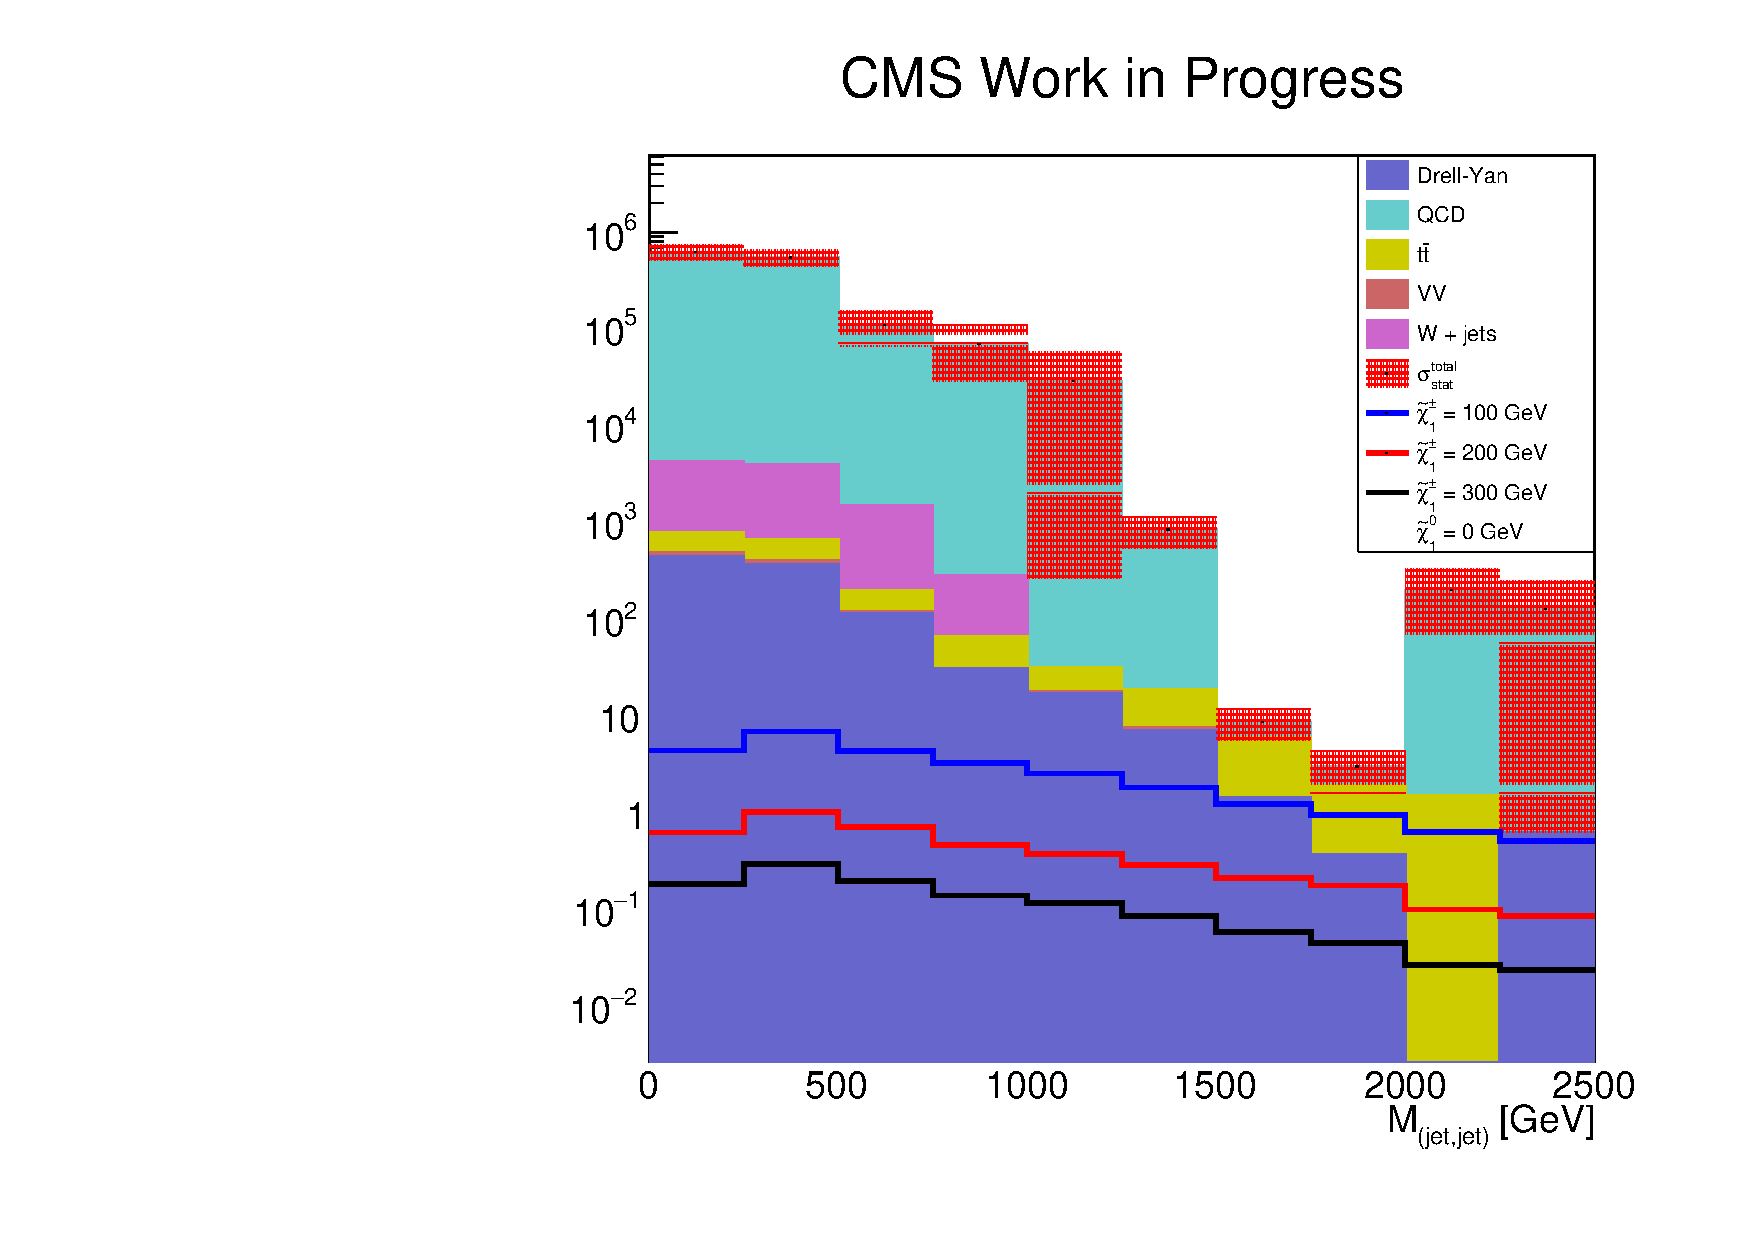
\includegraphics[width=0.5\textwidth]{analysis/pics/h_dijetinvariantmass_Taui2TightIso.pdf}
		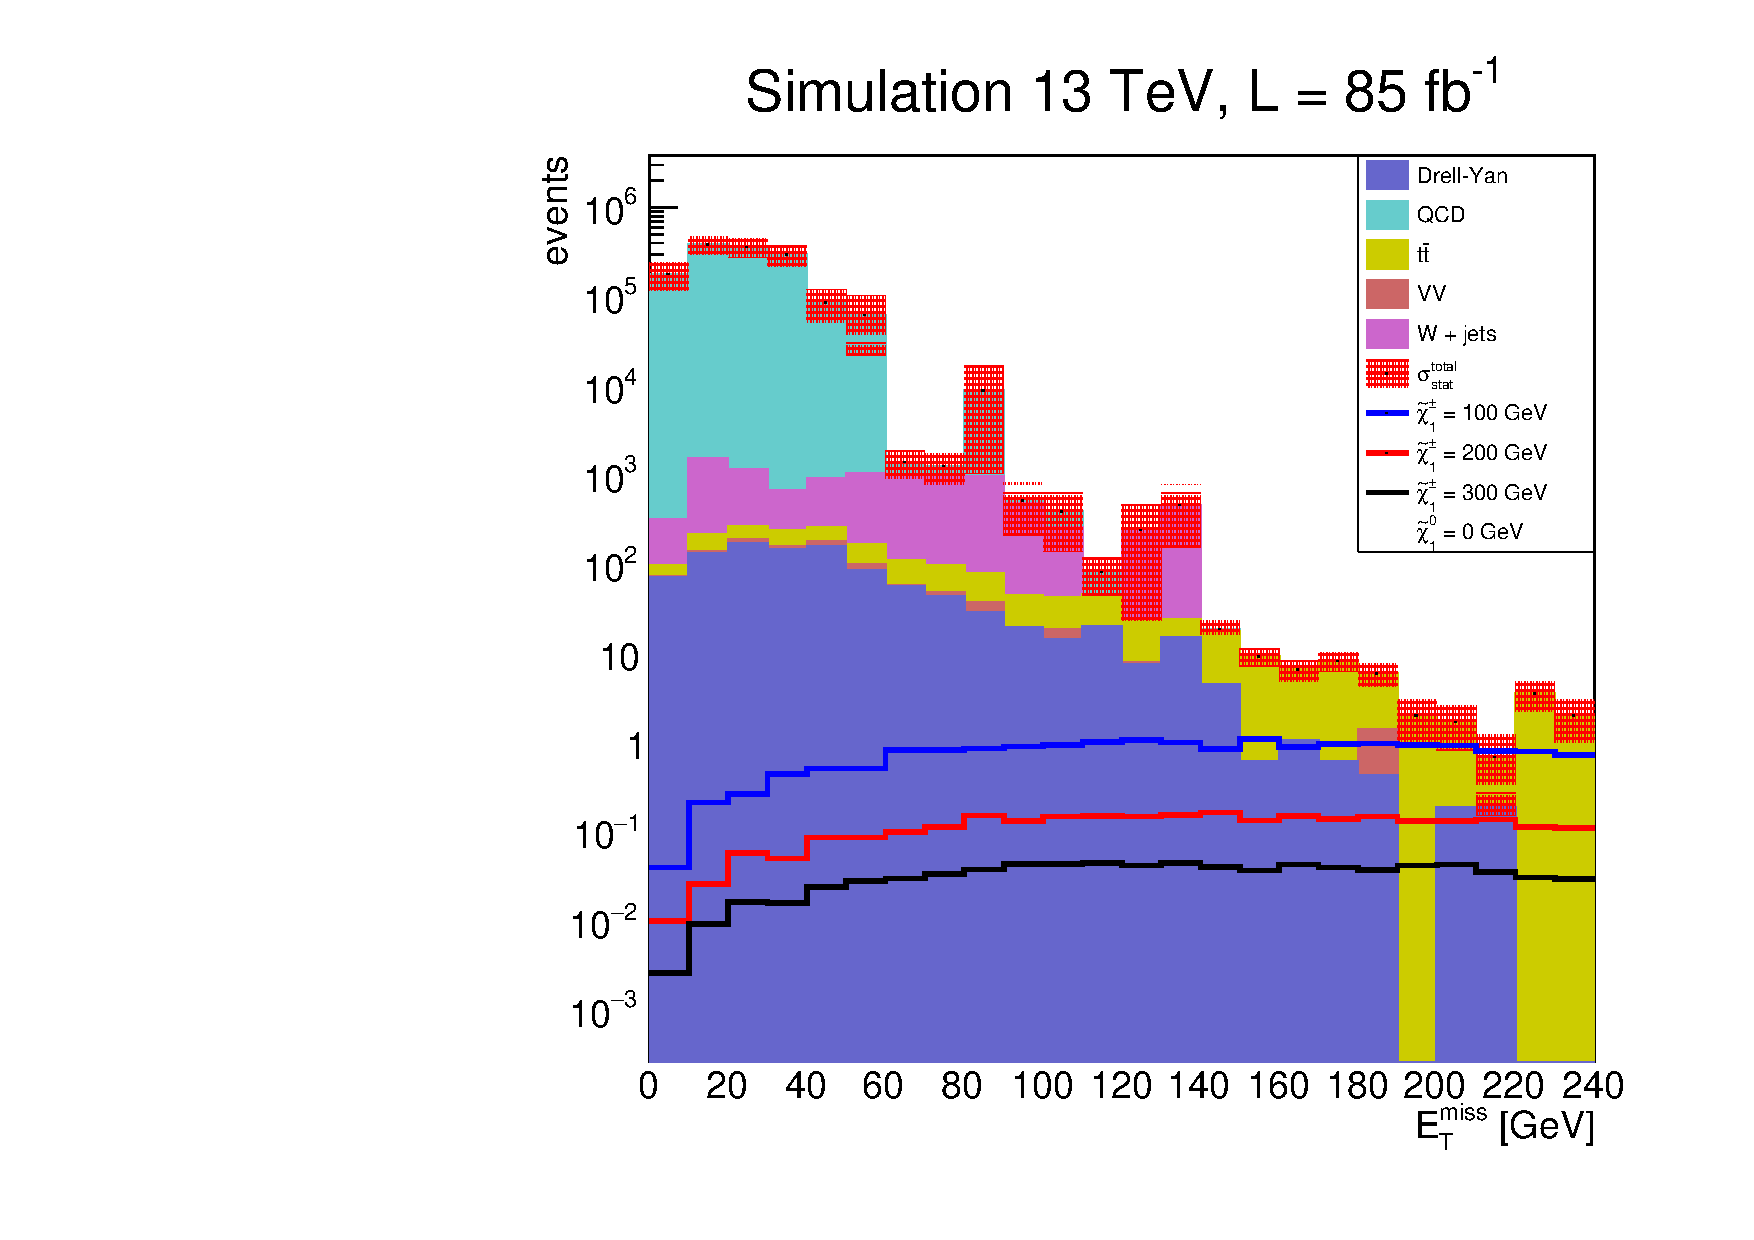
\includegraphics[width=0.5\textwidth]{analysis/pics/h_met_Taui2TightIso.pdf}
	\end{tabular}
	\caption{(Left) Di-jet invariant mass distribution and (Right) and \met distribution of selected signal and all MC background samples in signal region.}
	\label{fig::crplots1_Taui2TightIso_13tev}
\end{figure}

\begin{figure}[tbh!]
	\centering
	\begin{tabular}{cc}
		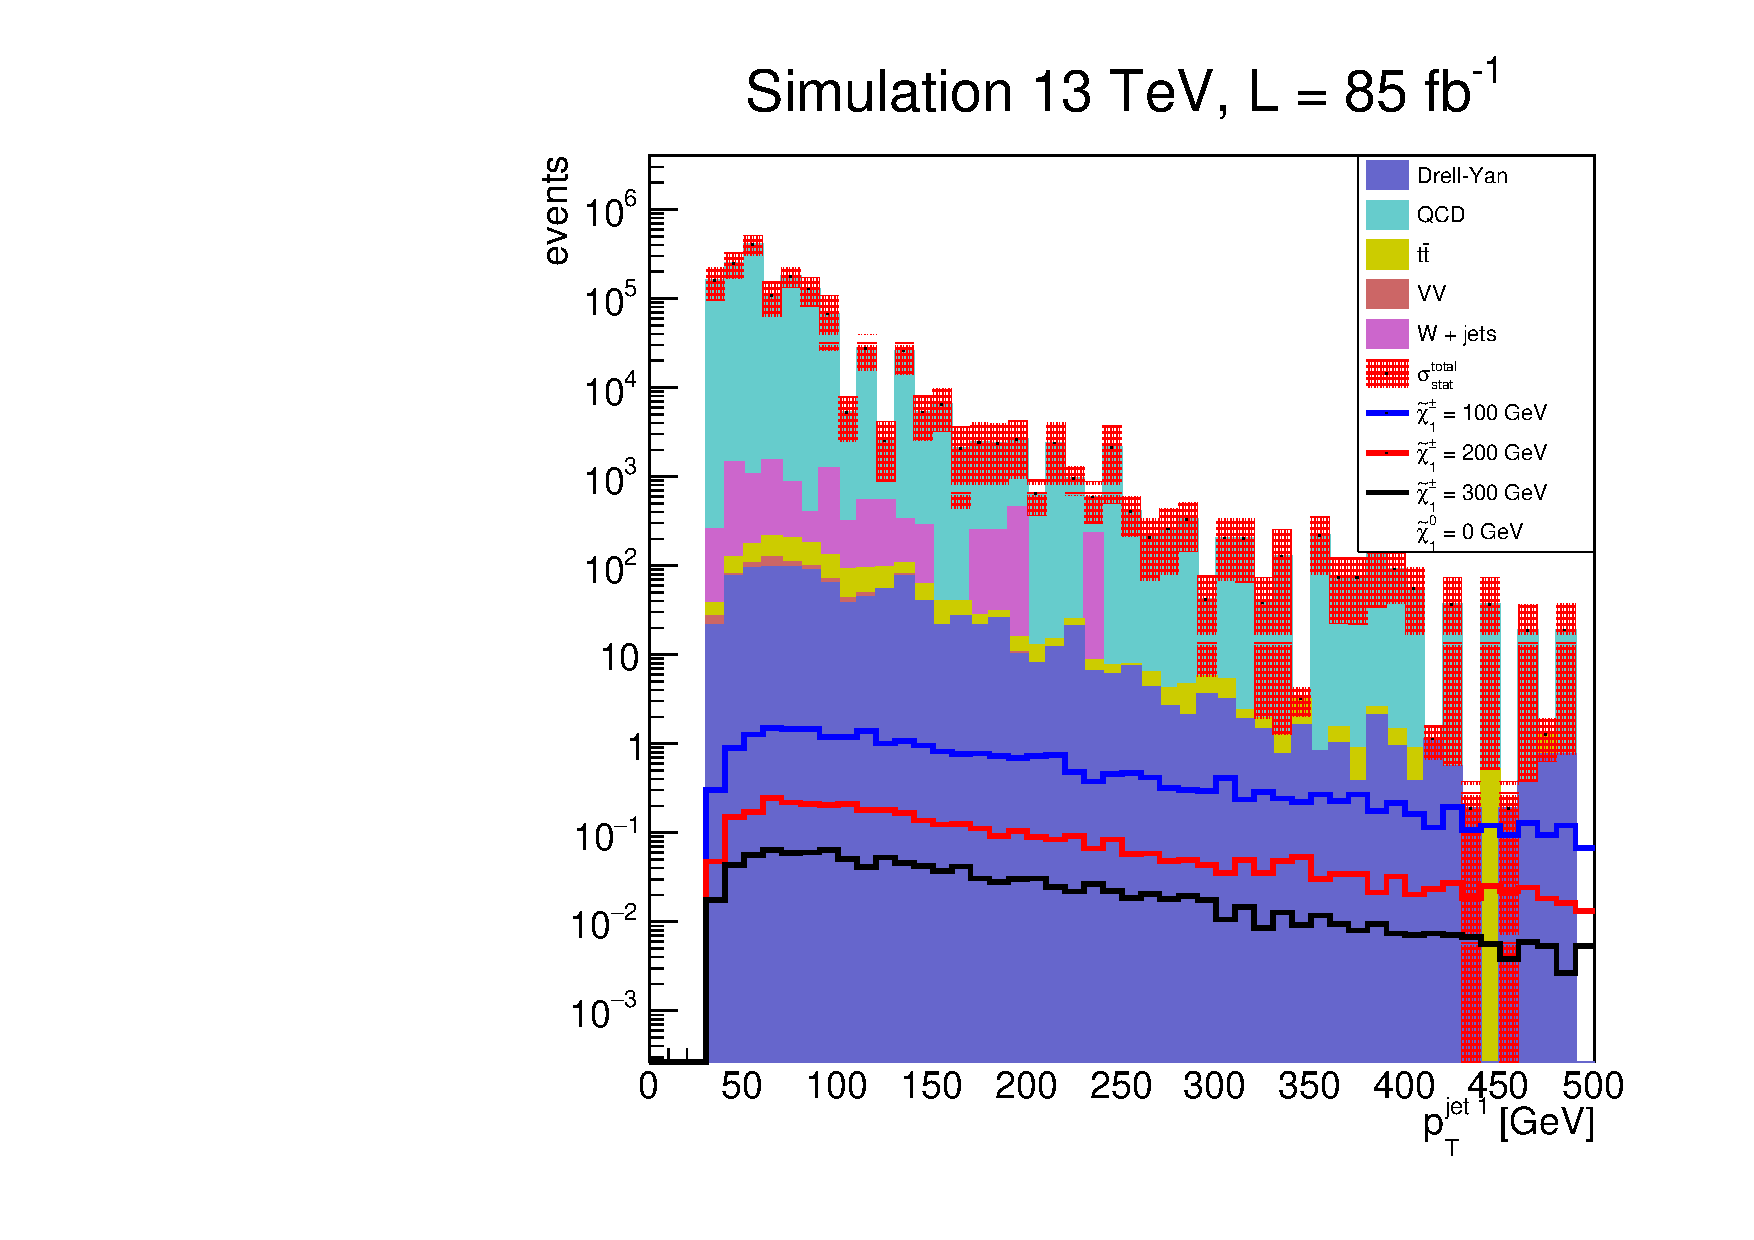
\includegraphics[width=0.5\textwidth]{analysis/pics/h_jet1pt_Taui2TightIso.pdf}
		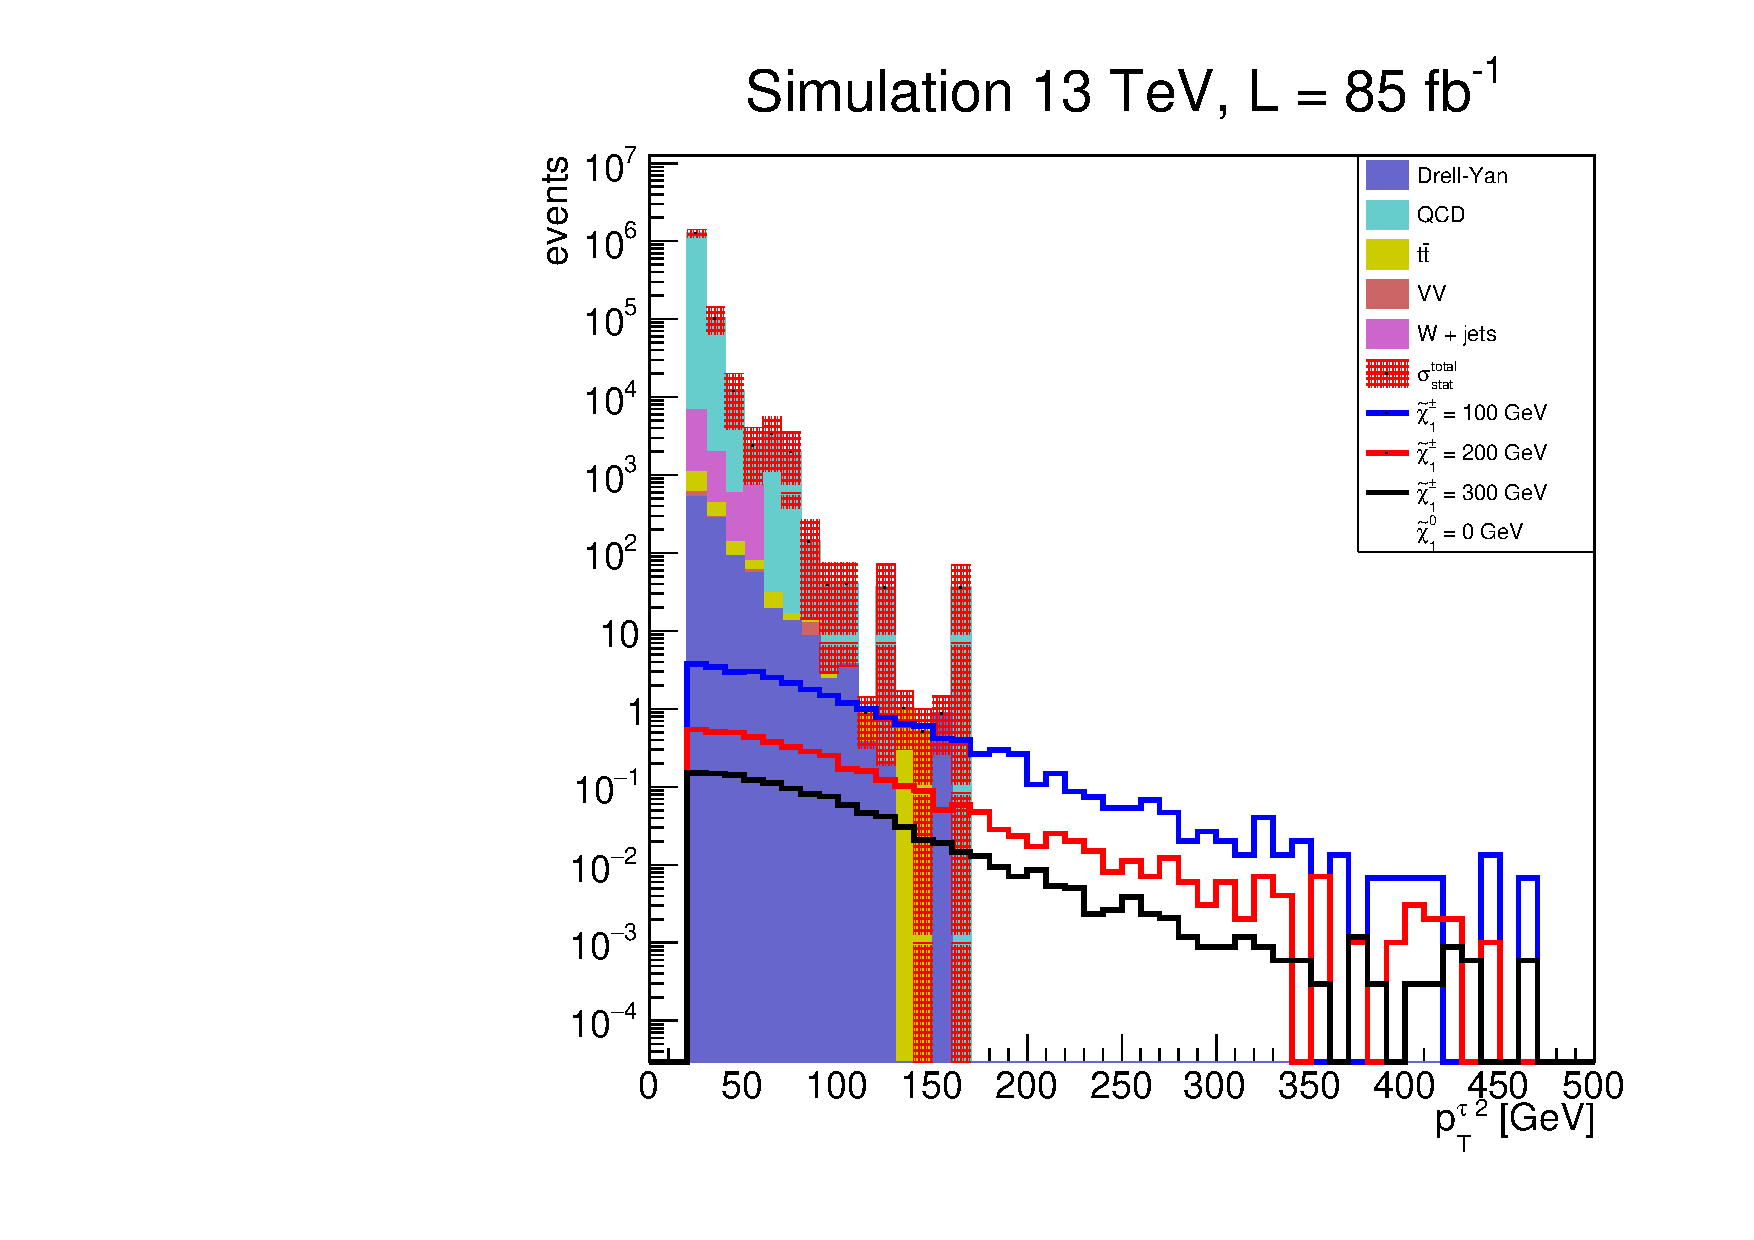
\includegraphics[width=0.5\textwidth]{analysis/pics/h_tau2pt_Taui2TightIso.pdf}
	\end{tabular}
	\caption{(Left) Leading jet \pt distribution and (Right) and second leading \hadtau \pt distribution of selected signal and all MC background samples in signal region.}
	\label{fig::crplots2_Taui2TightIso_13tev}
\end{figure}

\subsection*{Control region 2}

\FloatBarrier

2 tight-isolated \hadtau, inverted VBF selection

\begin{figure}[tbh!]
	\centering
	\begin{tabular}{cc}
		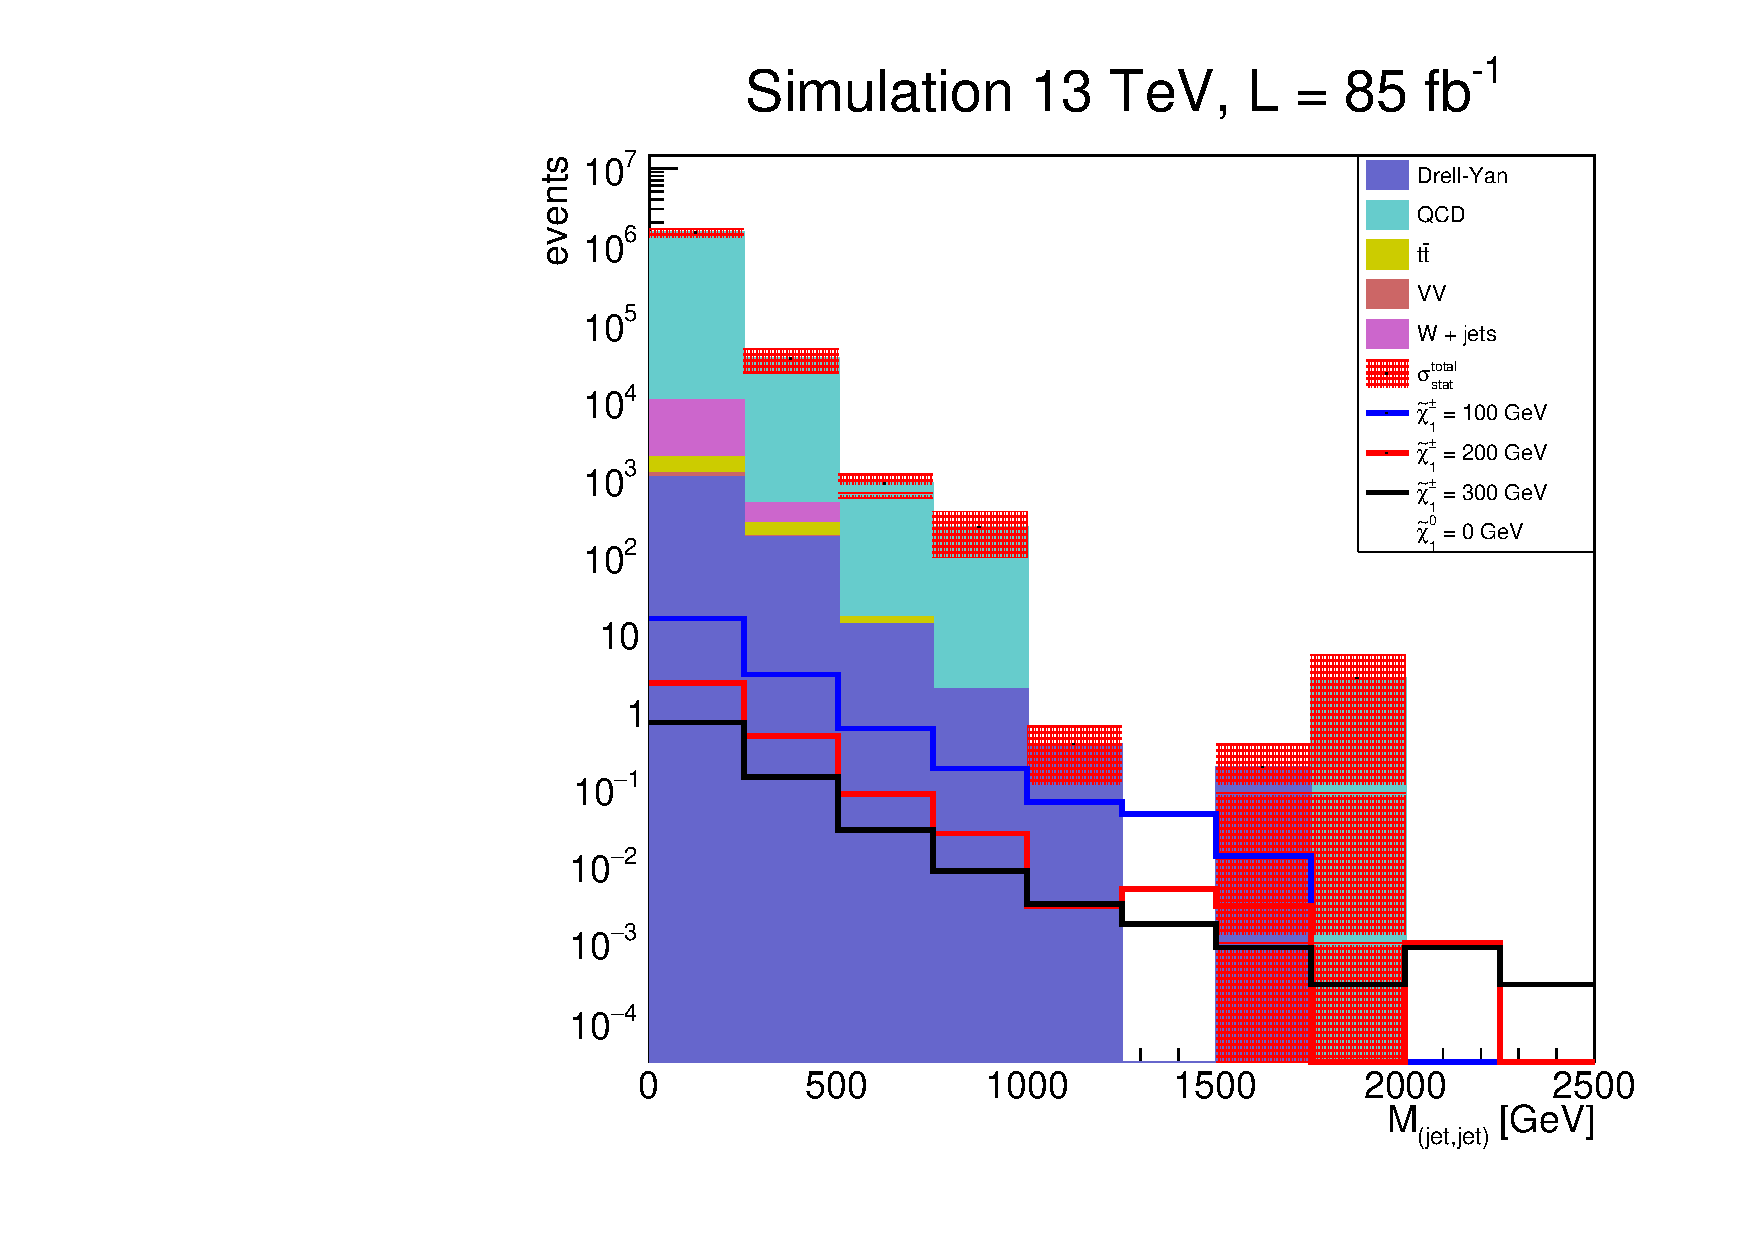
\includegraphics[width=0.5\textwidth]{analysis/pics/h_dijetinvariantmass_Tau2TightIsoVBFInverted.pdf}
		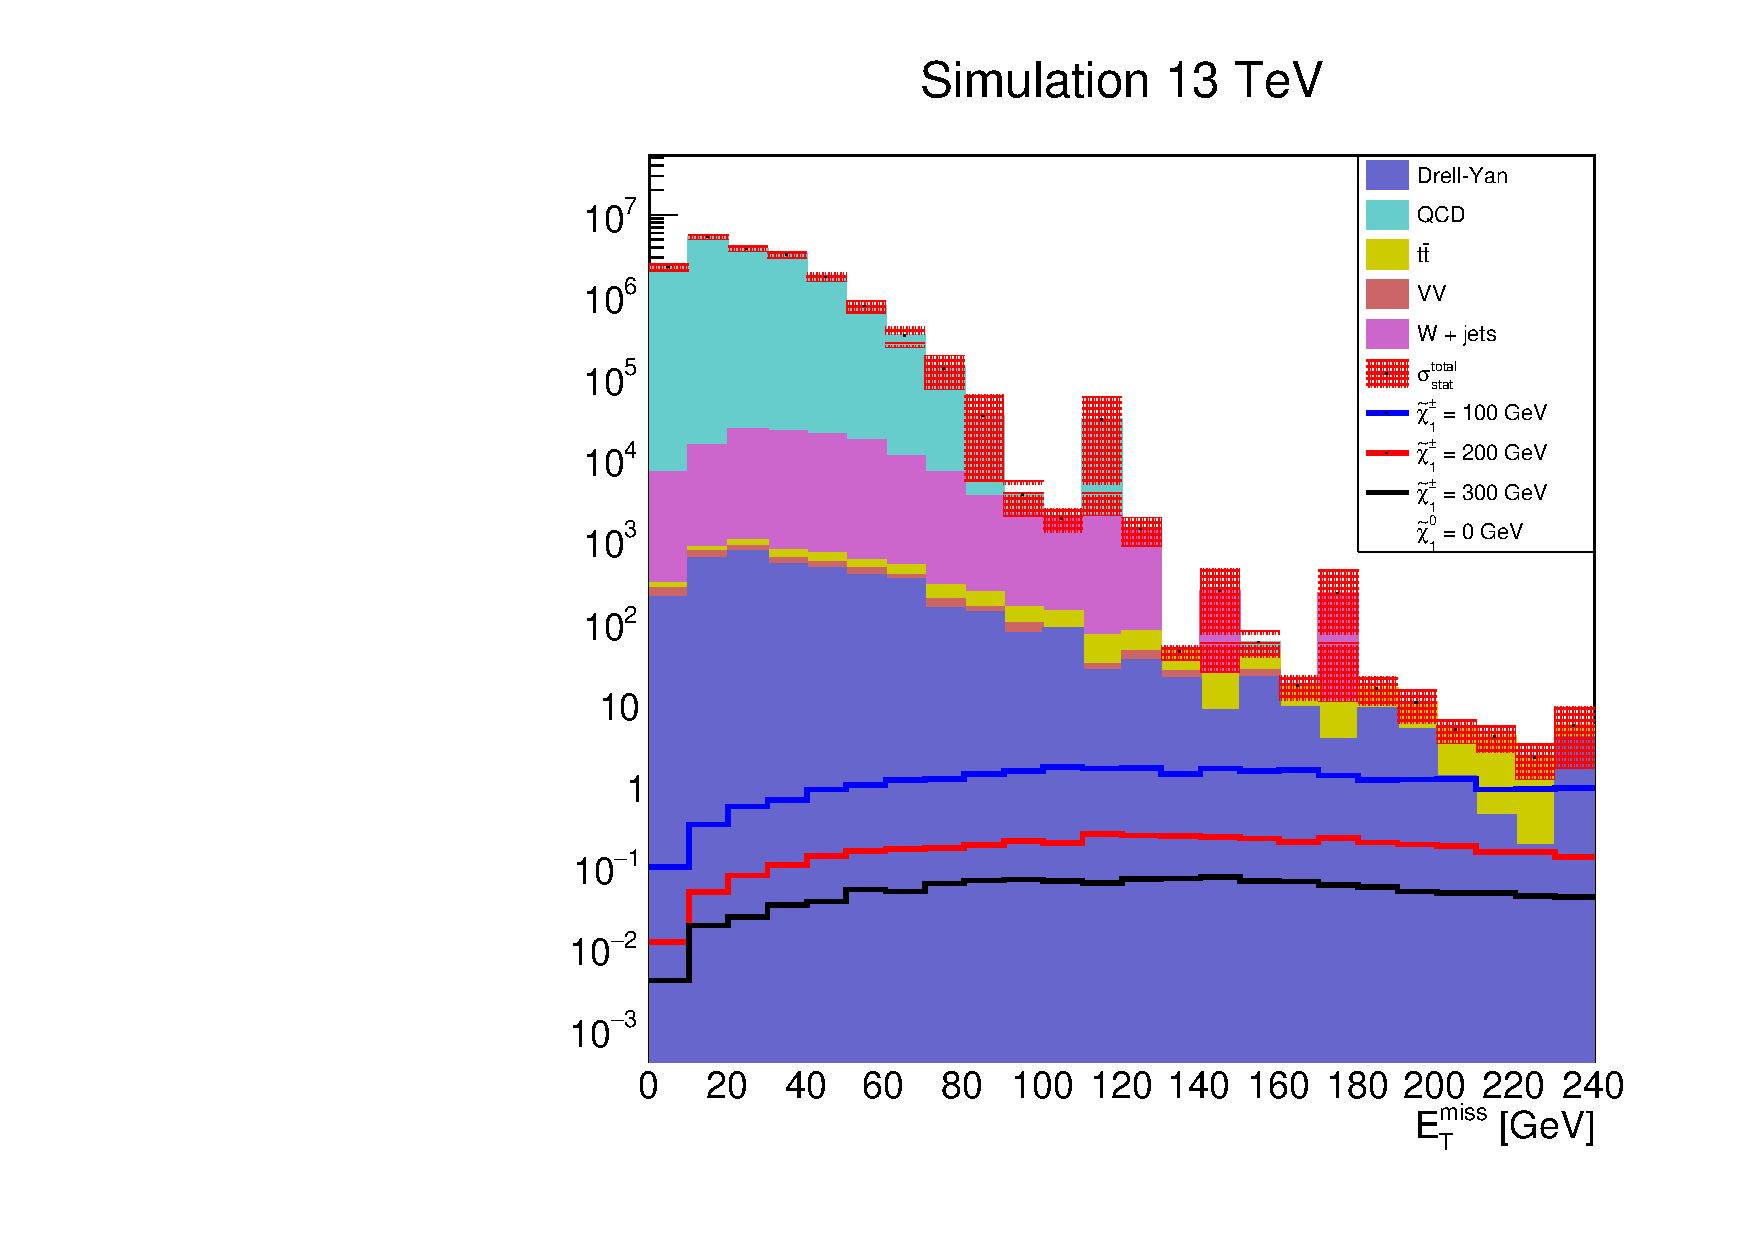
\includegraphics[width=0.5\textwidth]{analysis/pics/h_met_Tau2TightIsoVBFInverted.pdf}
	\end{tabular}
	\caption{(Left) Di-jet invariant mass distribution and (Right) and \met distribution of selected signal and all MC background samples in control region 2.}
	\label{fig::crplots1_Tau2TightIsoVBFInverted_13tev}
\end{figure}

\begin{figure}[tbh!]
	\centering
	\begin{tabular}{cc}
		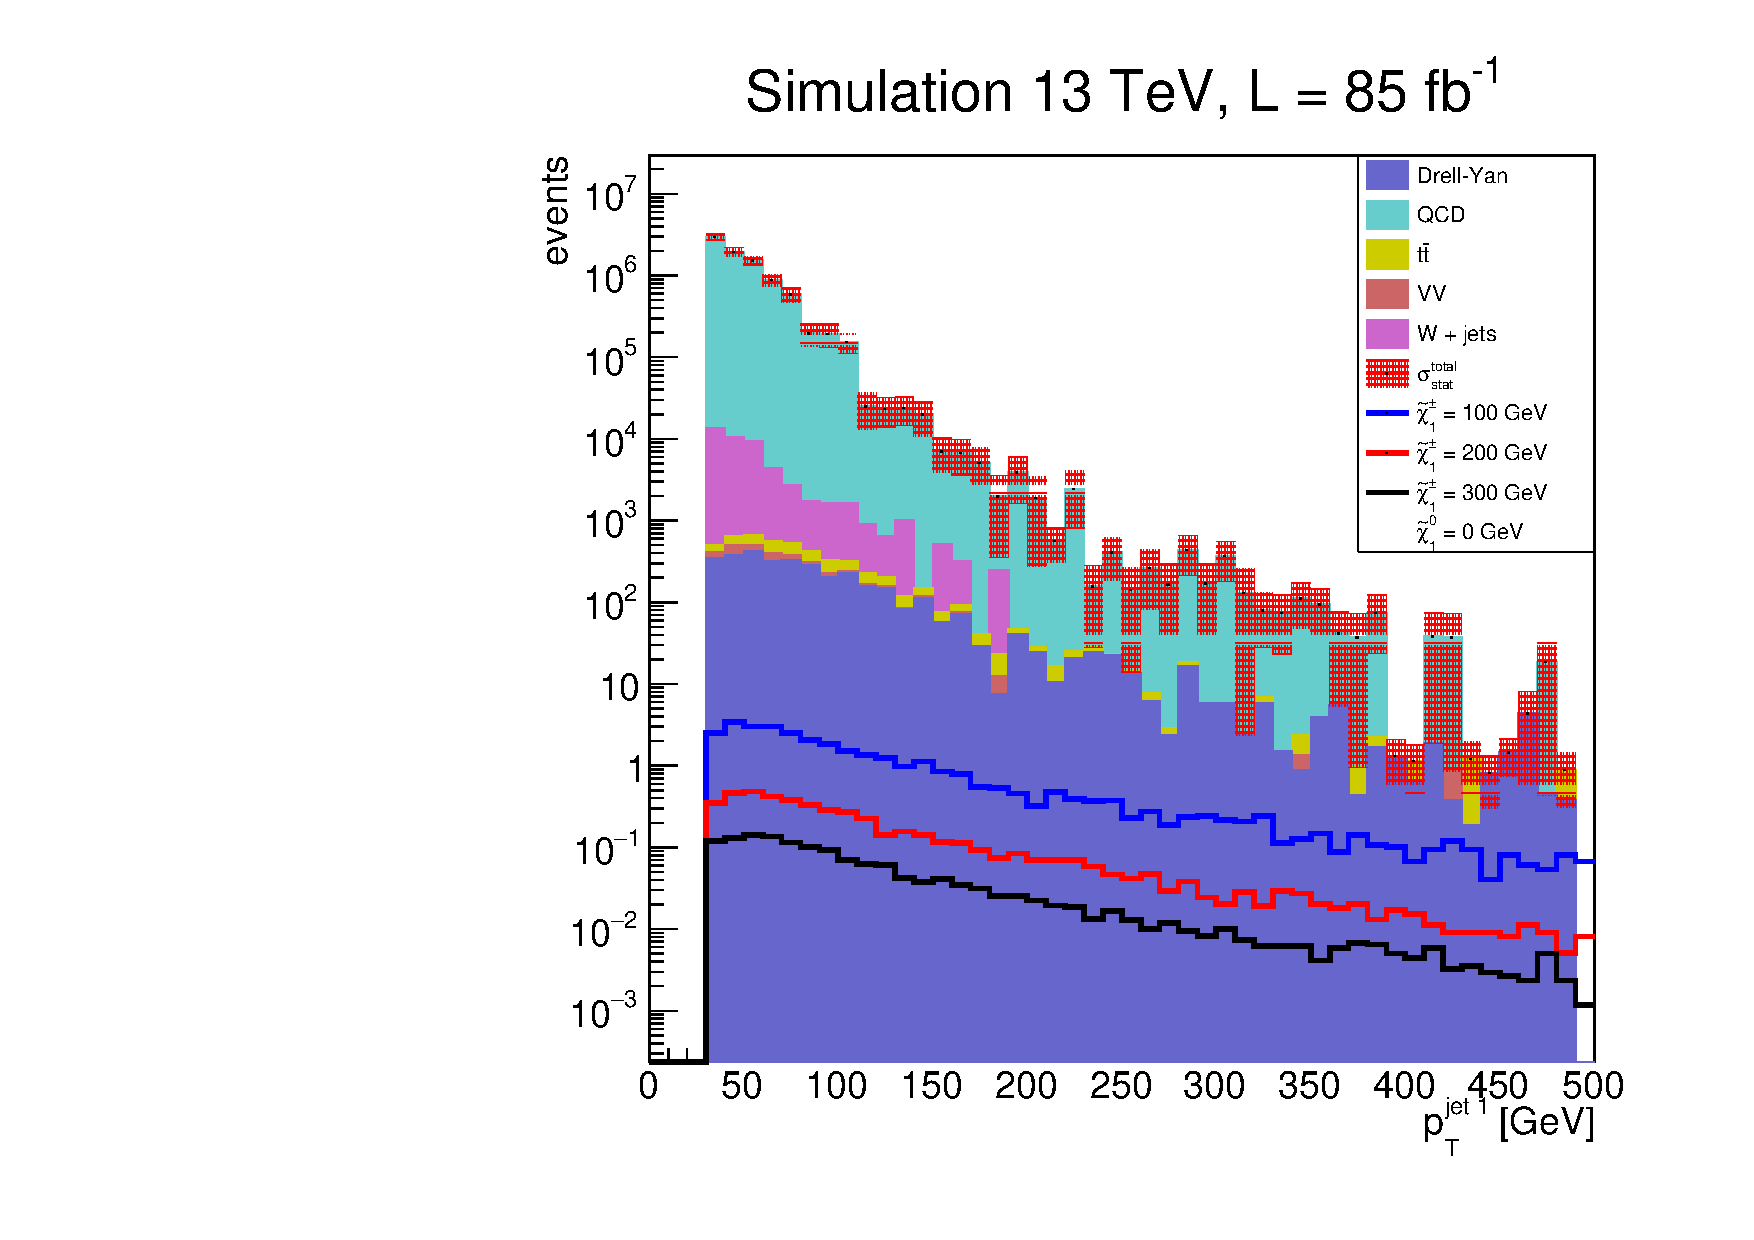
\includegraphics[width=0.5\textwidth]{analysis/pics/h_jet1pt_Tau2TightIsoVBFInverted.pdf}
		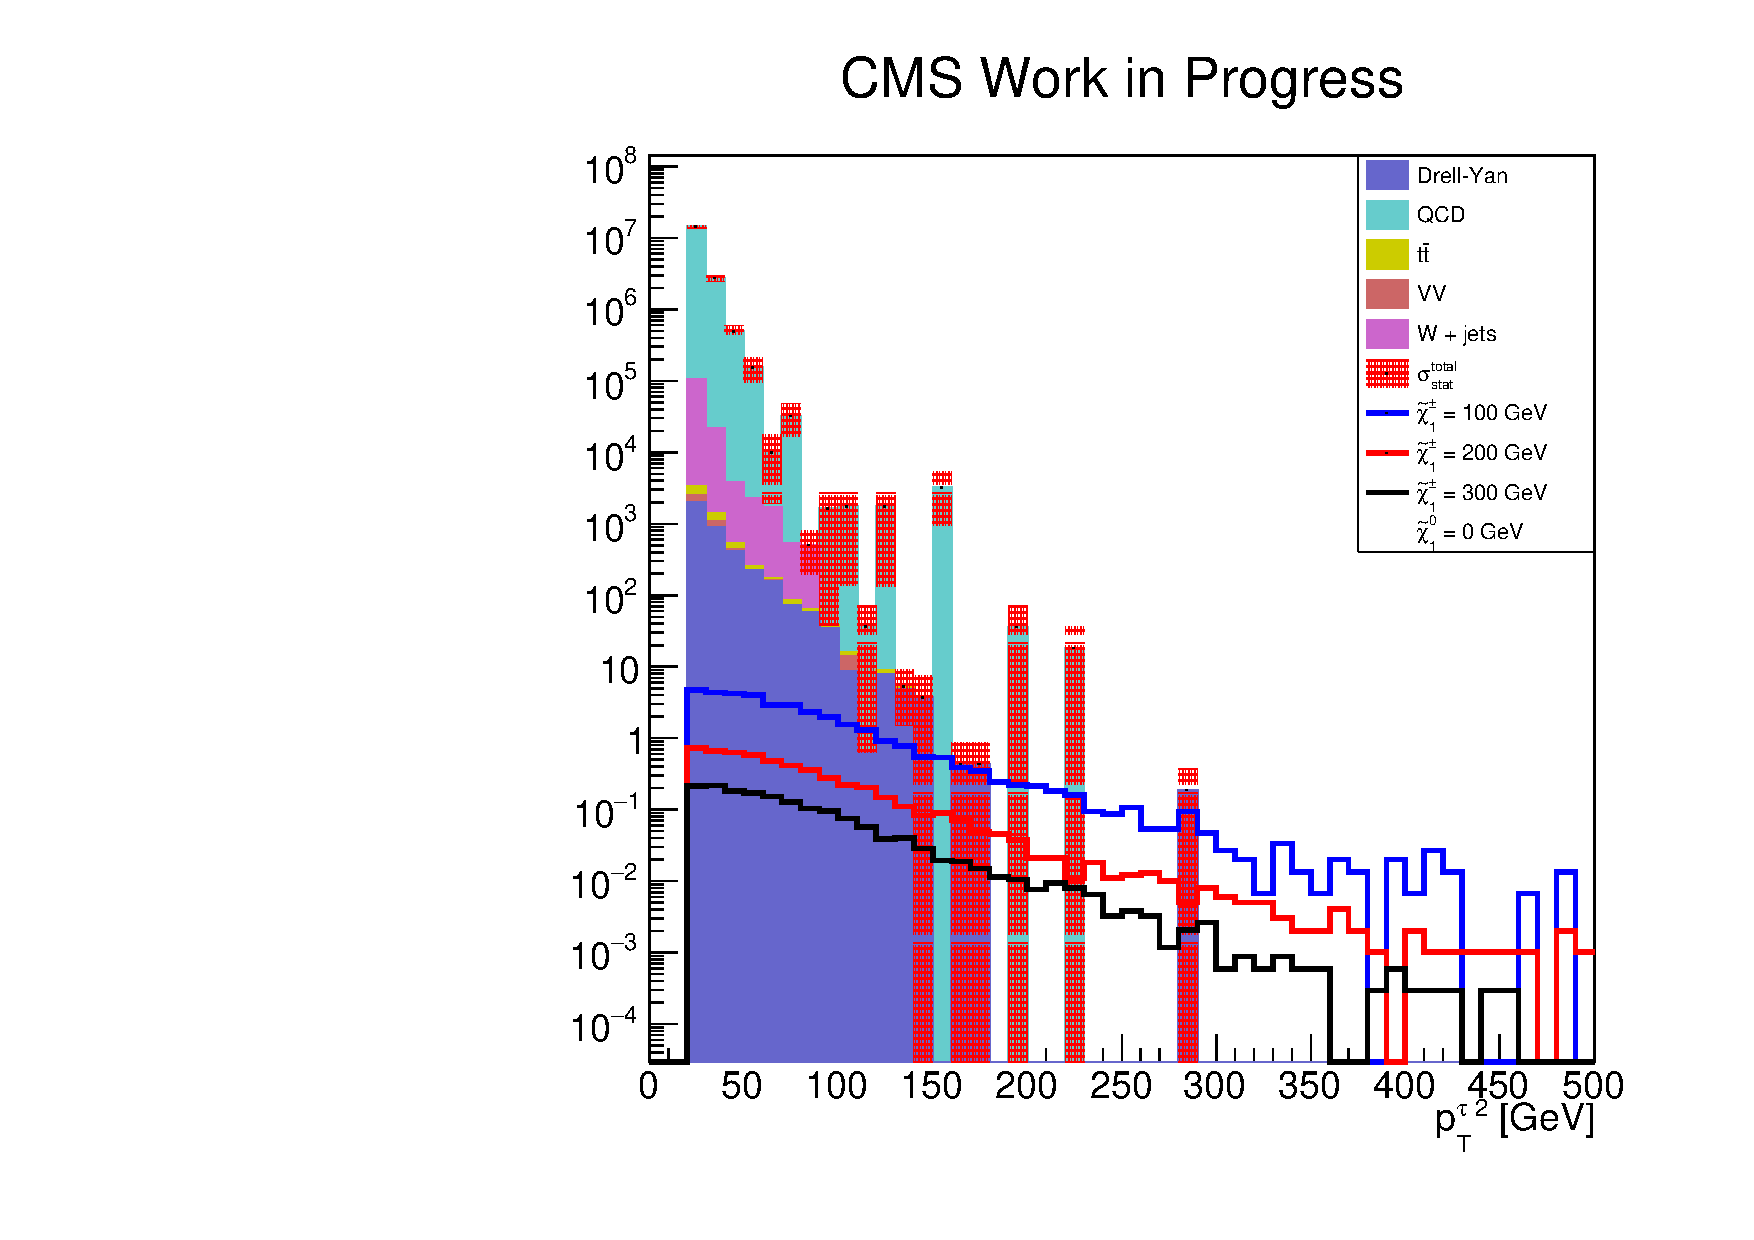
\includegraphics[width=0.5\textwidth]{analysis/pics/h_tau2pt_Tau2TightIsoVBFInverted.pdf}
	\end{tabular}
	\caption{(Left) Leading jet \pt distribution and (Right) and second leading \hadtau \pt distribution of selected signal and all MC background samples in control region 2.}
	\label{fig::crplots2_Taui2TightIsoVBFInverted_13tev}
\end{figure}

\subsection*{Control region 3}

\FloatBarrier

2 loose-isolated \hadtau (inclusive)

\begin{figure}[tbh!]
	\centering
	\begin{tabular}{cc}
		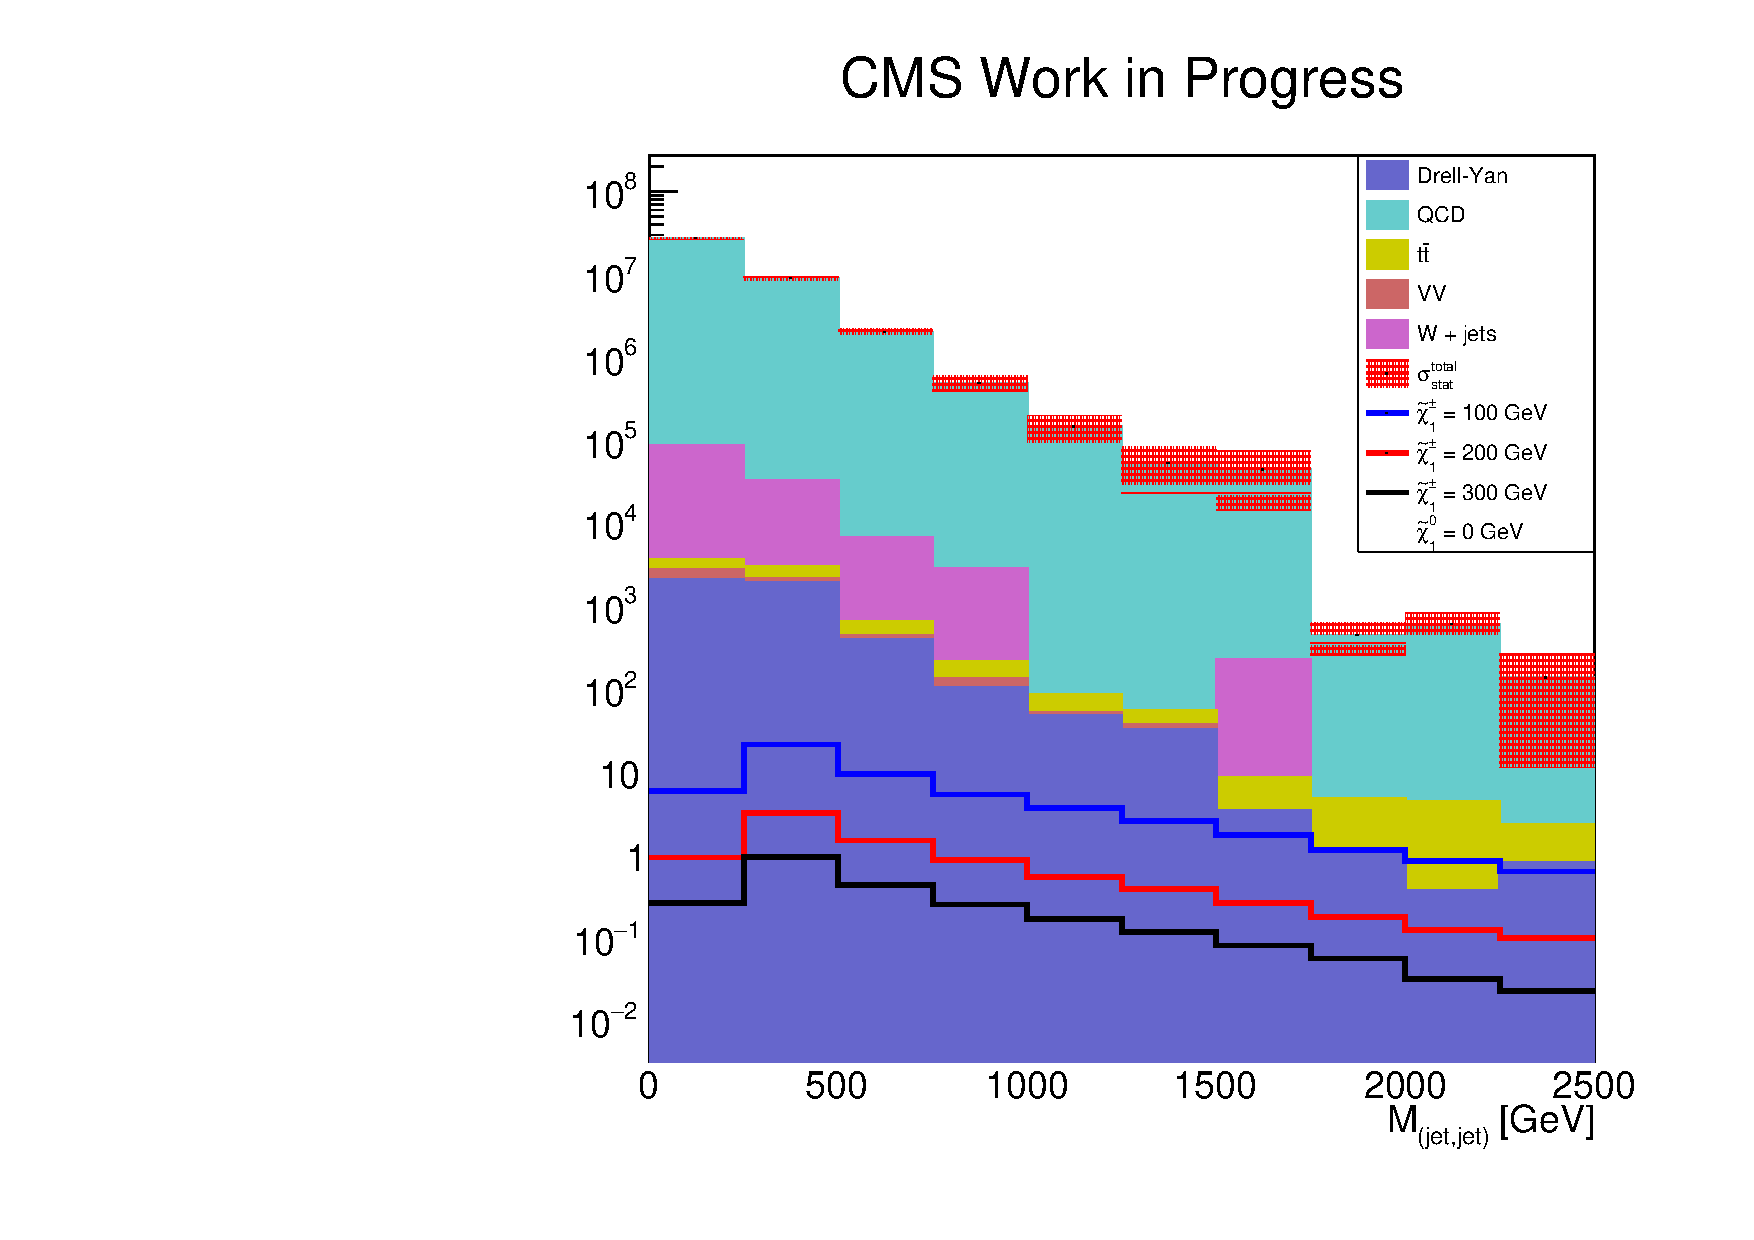
\includegraphics[width=0.5\textwidth]{analysis/pics/h_dijetinvariantmass_Tau2LooseIsoInclusive.pdf}
		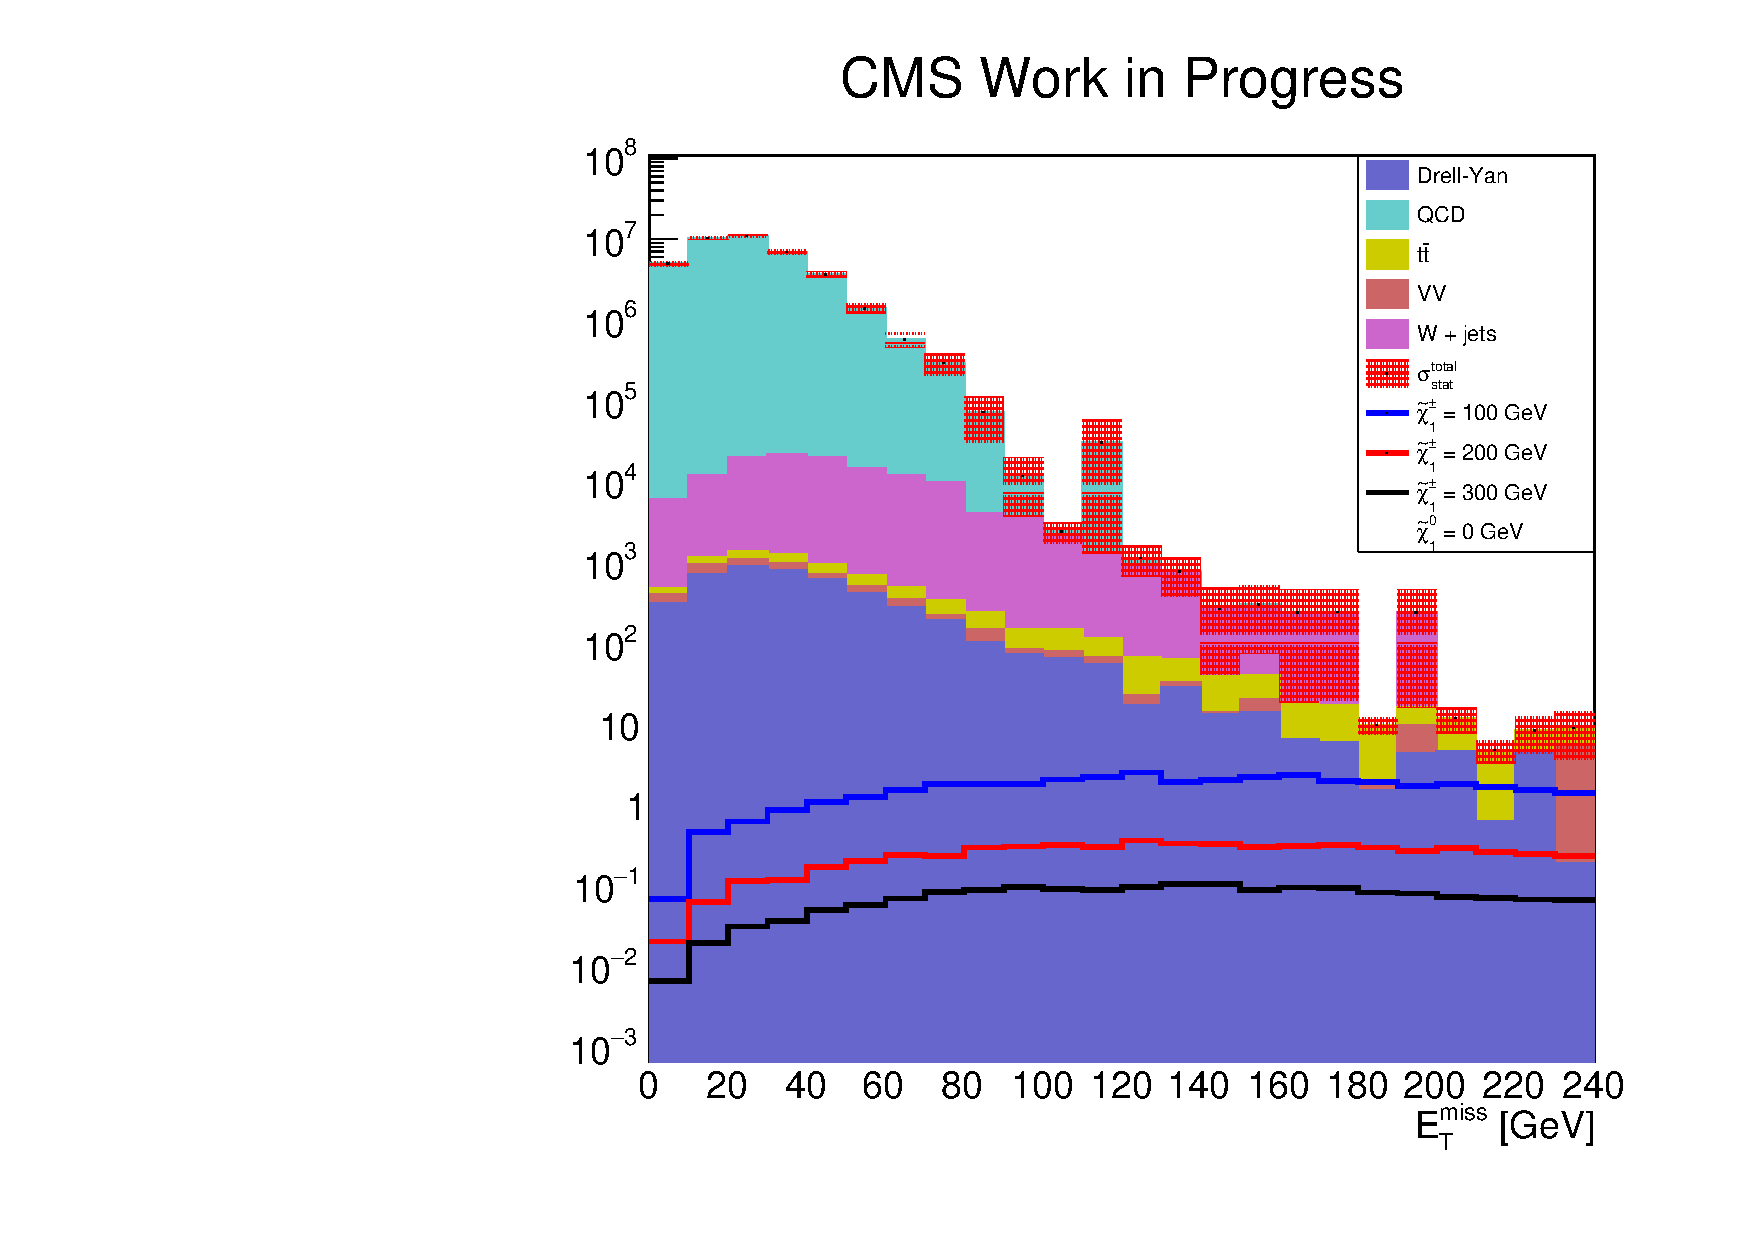
\includegraphics[width=0.5\textwidth]{analysis/pics/h_met_Tau2LooseIsoInclusive.pdf}
	\end{tabular}
	\caption{(Left) Di-jet invariant mass distribution and (Right) and \met distribution of selected signal and all MC background samples in control region 3.}
	\label{fig::crplots1_Tau2LooseIsoInclusive_13tev}
\end{figure}

\begin{figure}[tbh!]
	\centering
	\begin{tabular}{cc}
		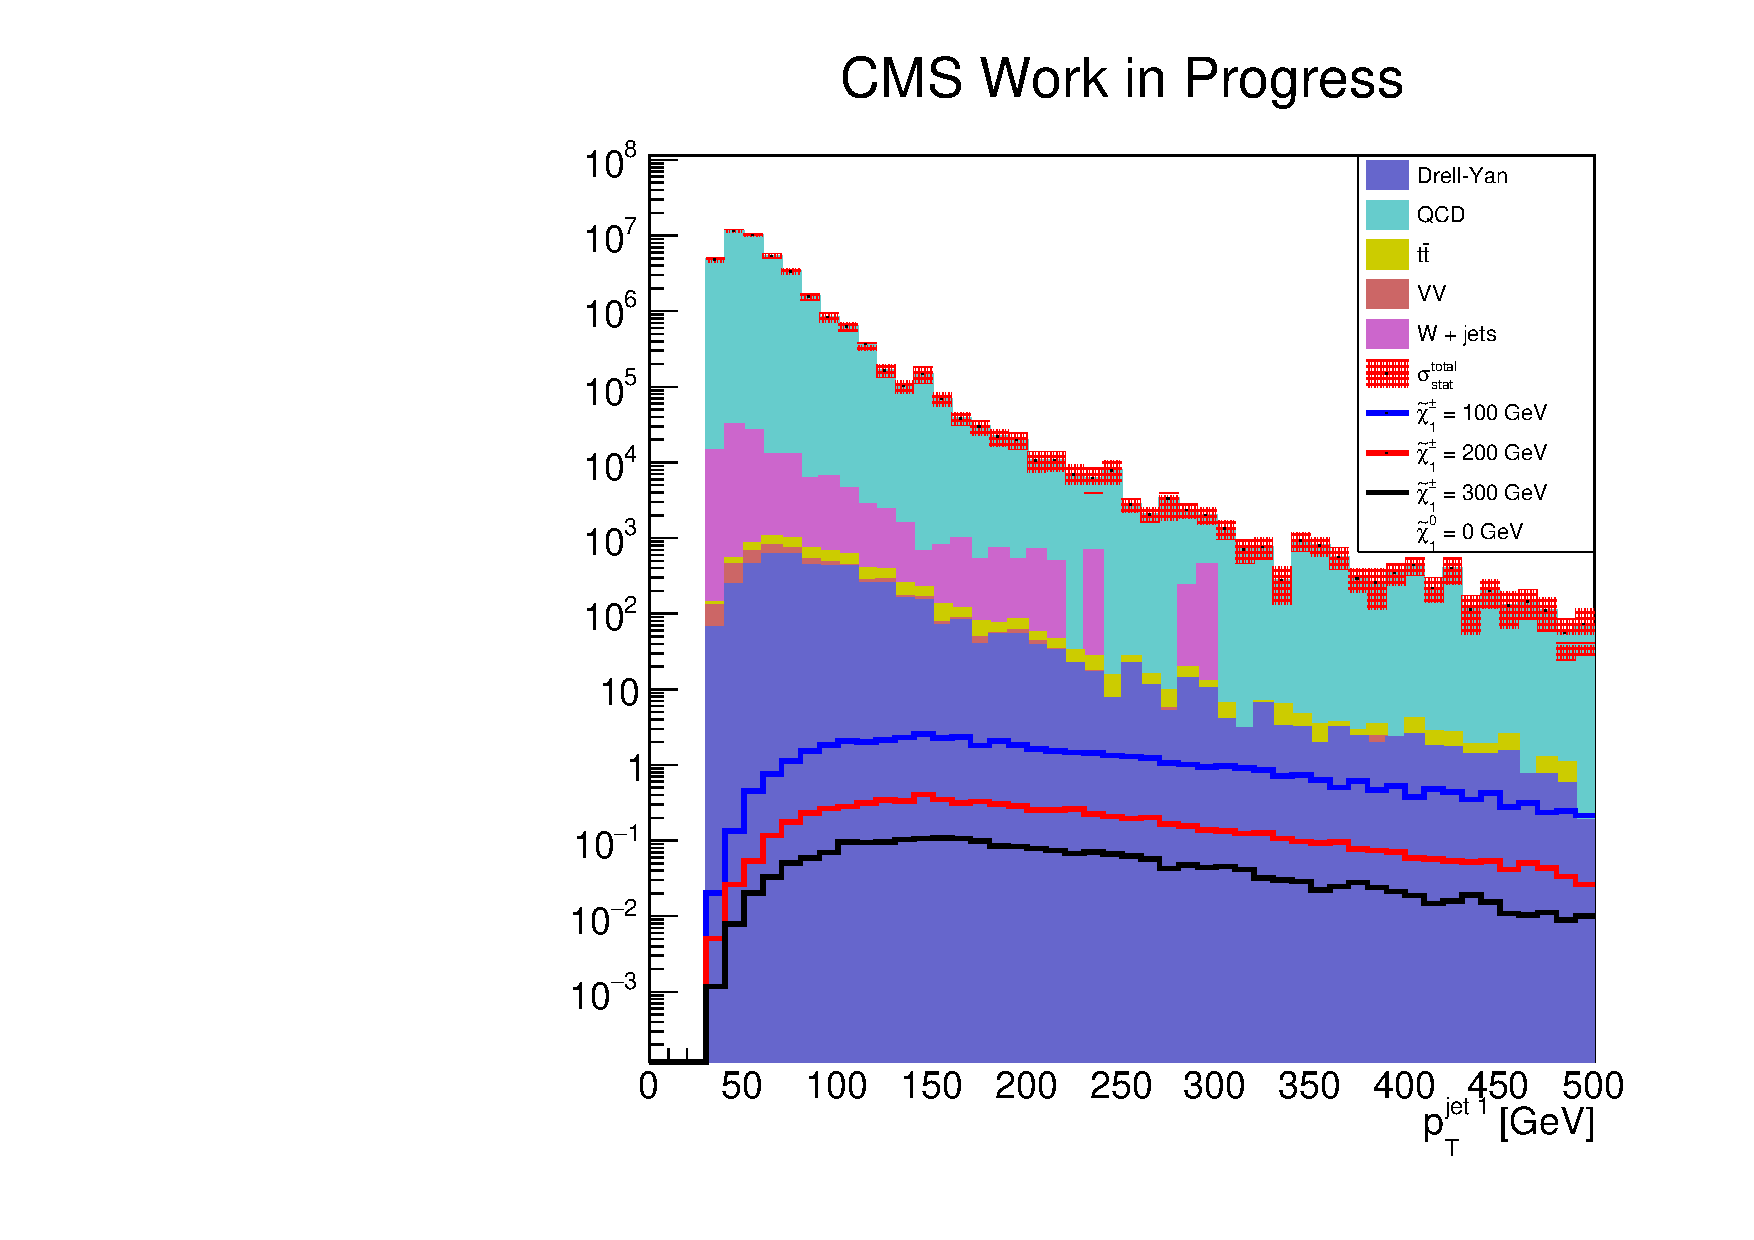
\includegraphics[width=0.5\textwidth]{analysis/pics/h_jet1pt_Tau2LooseIsoInclusive.pdf}
		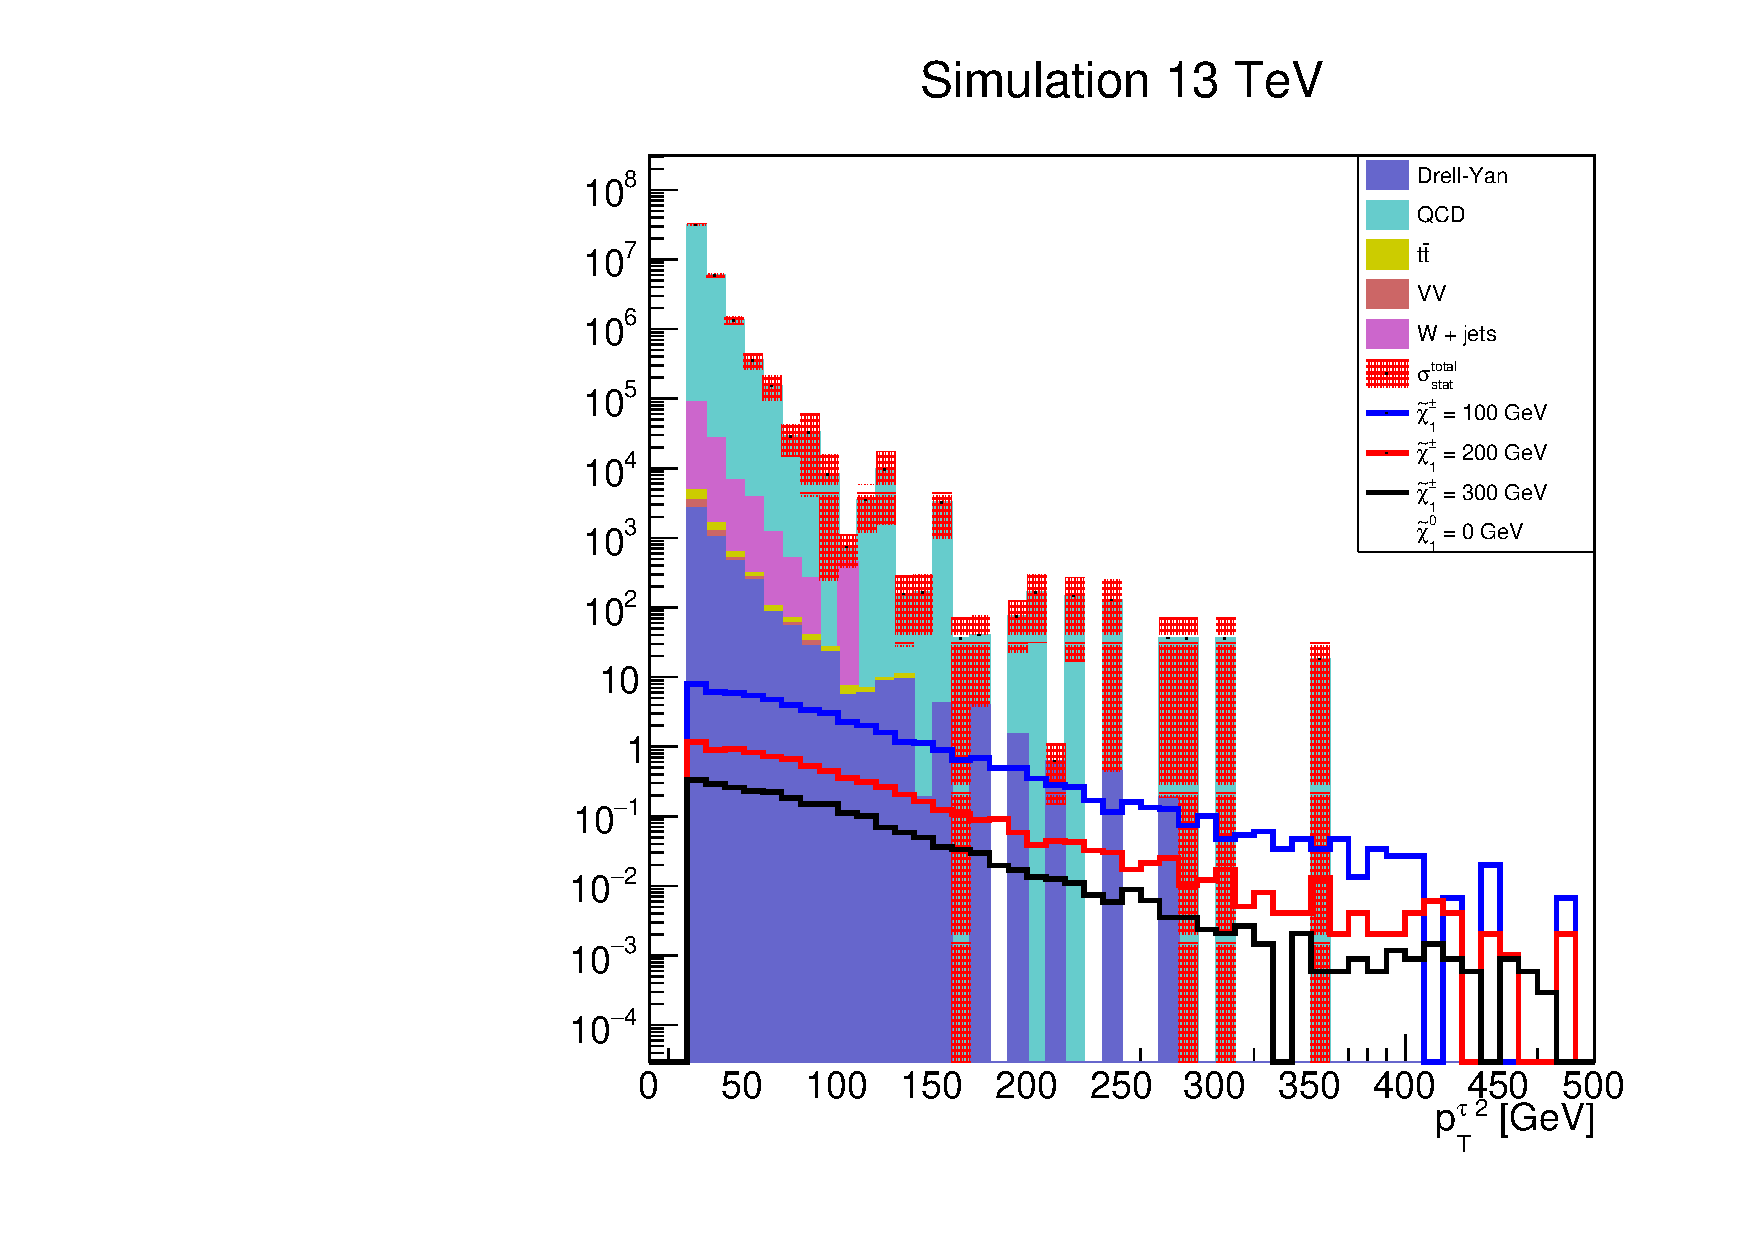
\includegraphics[width=0.5\textwidth]{analysis/pics/h_tau2pt_Tau2LooseIsoInclusive.pdf}
	\end{tabular}
	\caption{(Left) Leading jet \pt distribution and (Right) and second leading \hadtau \pt distribution of selected signal and all MC background samples in control region 3.}
	\label{fig::crplots2_Tau2LooseIsoInclusive_13tev}
\end{figure}

\subsection*{Control region 4}

\FloatBarrier

2 loose-isolated \hadtau (inclusive), inverted VBF selection

\begin{figure}[tbh!]
	\centering
	\begin{tabular}{cc}
		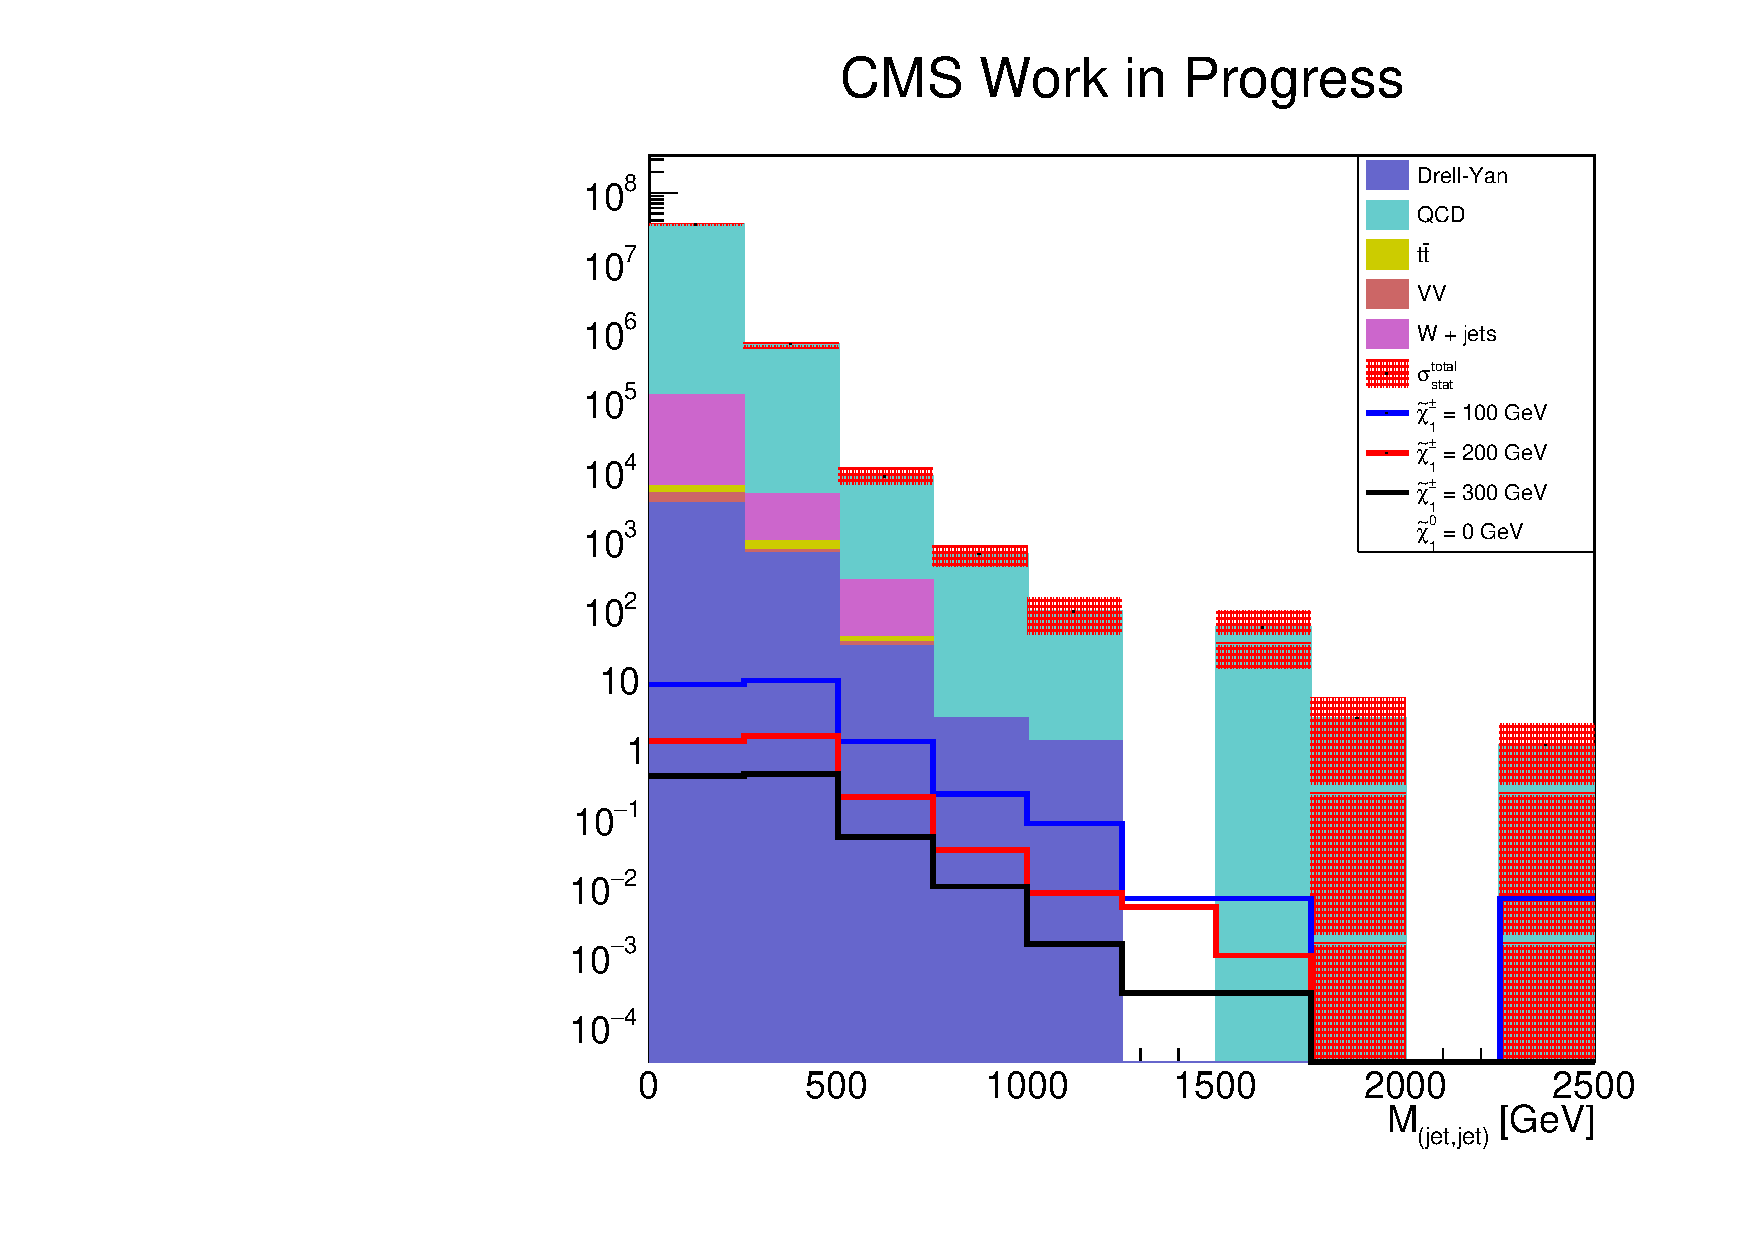
\includegraphics[width=0.5\textwidth]{analysis/pics/h_dijetinvariantmass_Tau2LooseIsoInclusiveVBFInverted.pdf}
		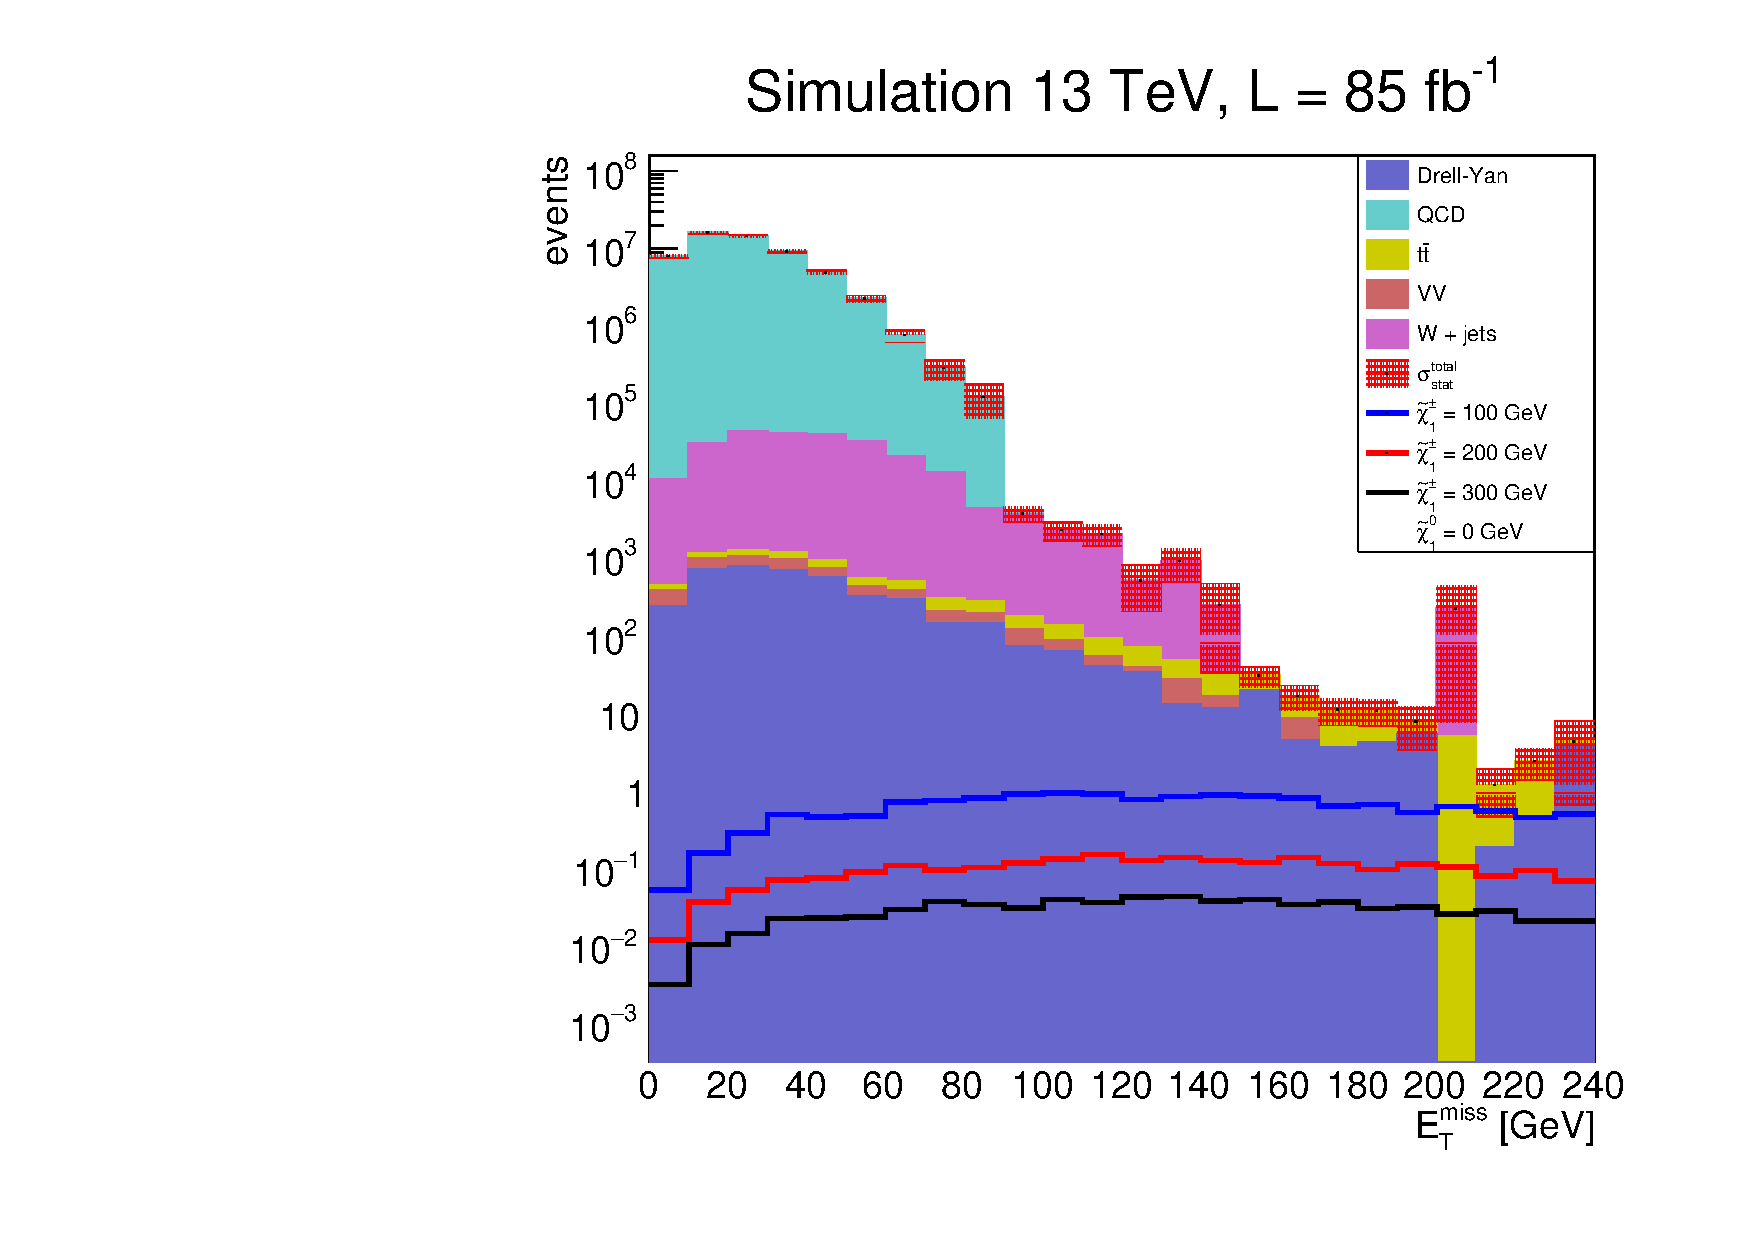
\includegraphics[width=0.5\textwidth]{analysis/pics/h_met_Tau2LooseIsoInclusiveVBFInverted.pdf}
	\end{tabular}
	\caption{(Left) Di-jet invariant mass distribution and (Right) and \met distribution of selected signal and all MC background samples in control region 4.}
	\label{fig::crplots1_Tau2LooseIsoInclusiveVBFInverted_13tev}
\end{figure}

\begin{figure}[tbh!]
	\centering
	\begin{tabular}{cc}
		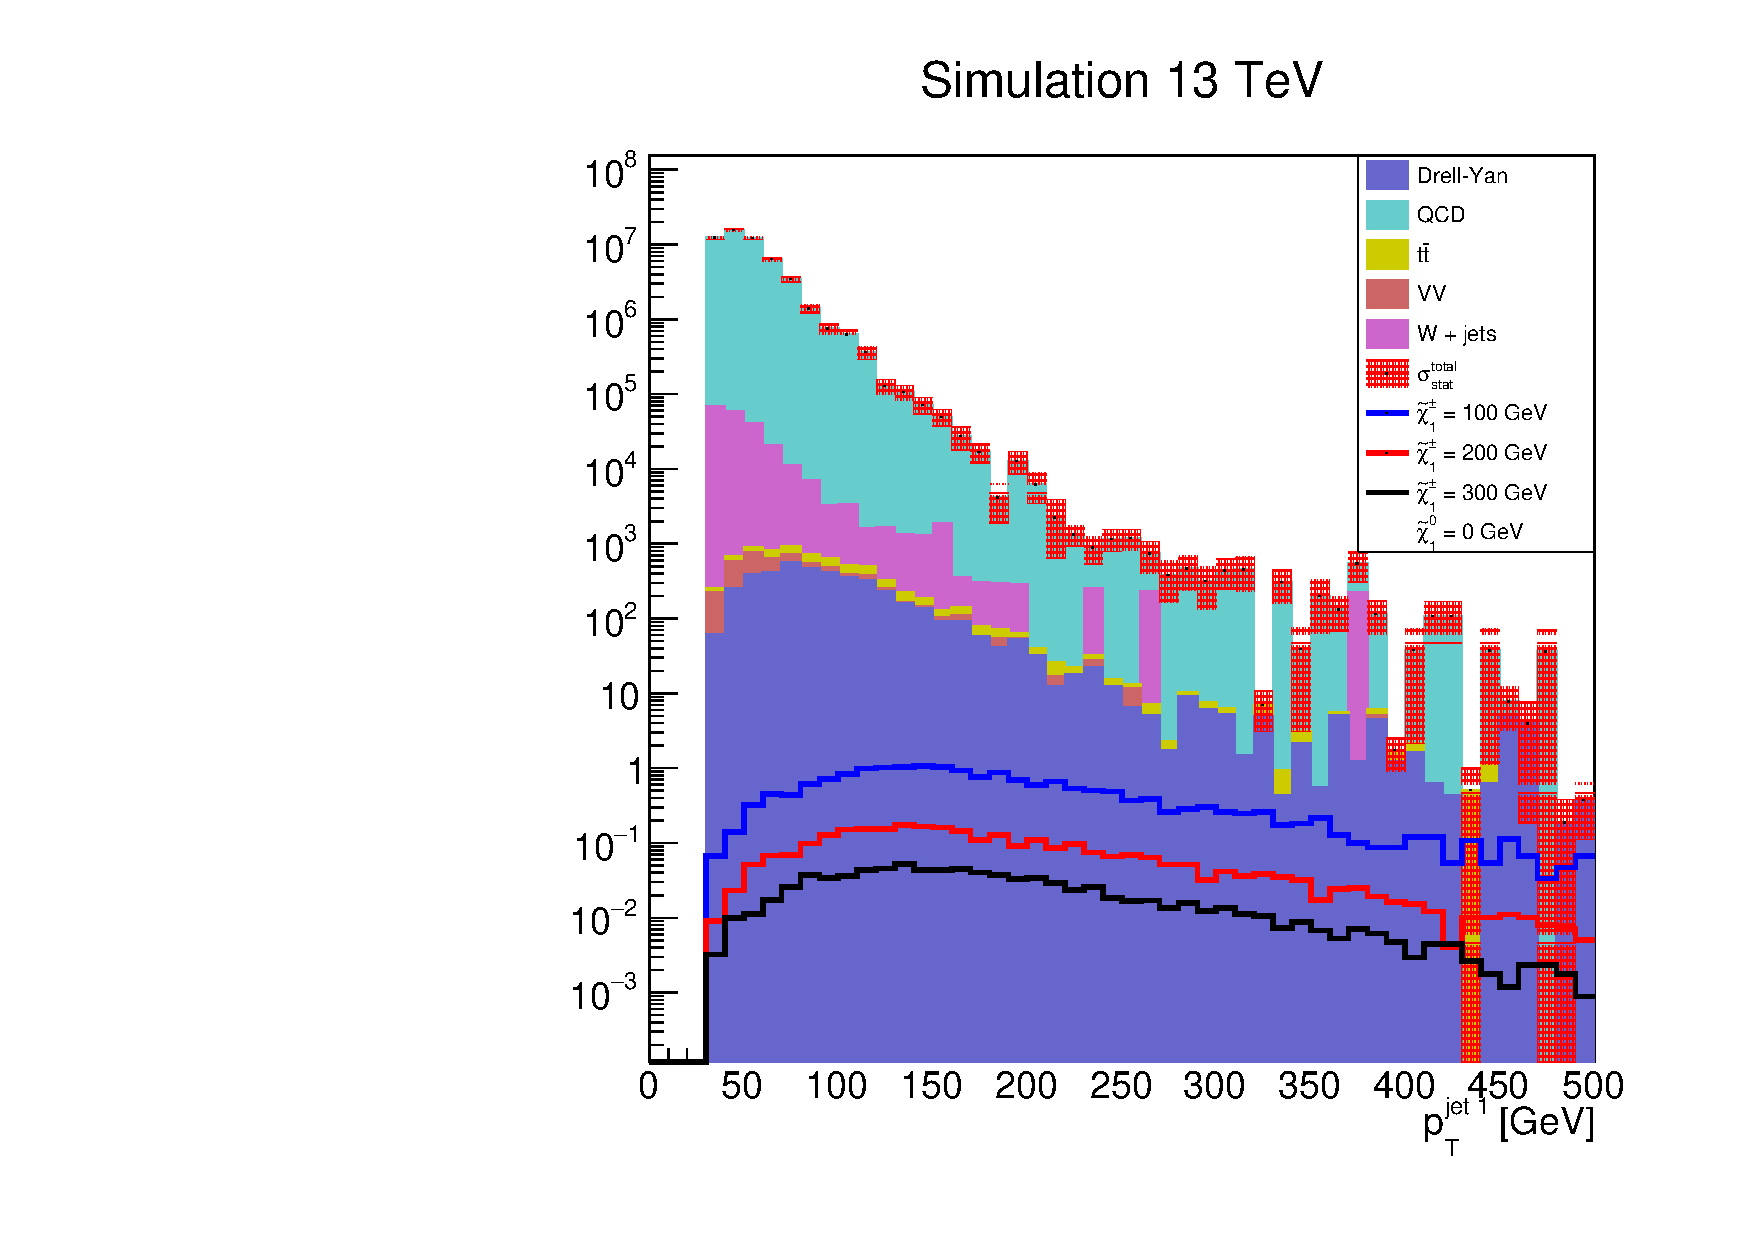
\includegraphics[width=0.5\textwidth]{analysis/pics/h_jet1pt_Tau2LooseIsoInclusiveVBFInverted.pdf}
		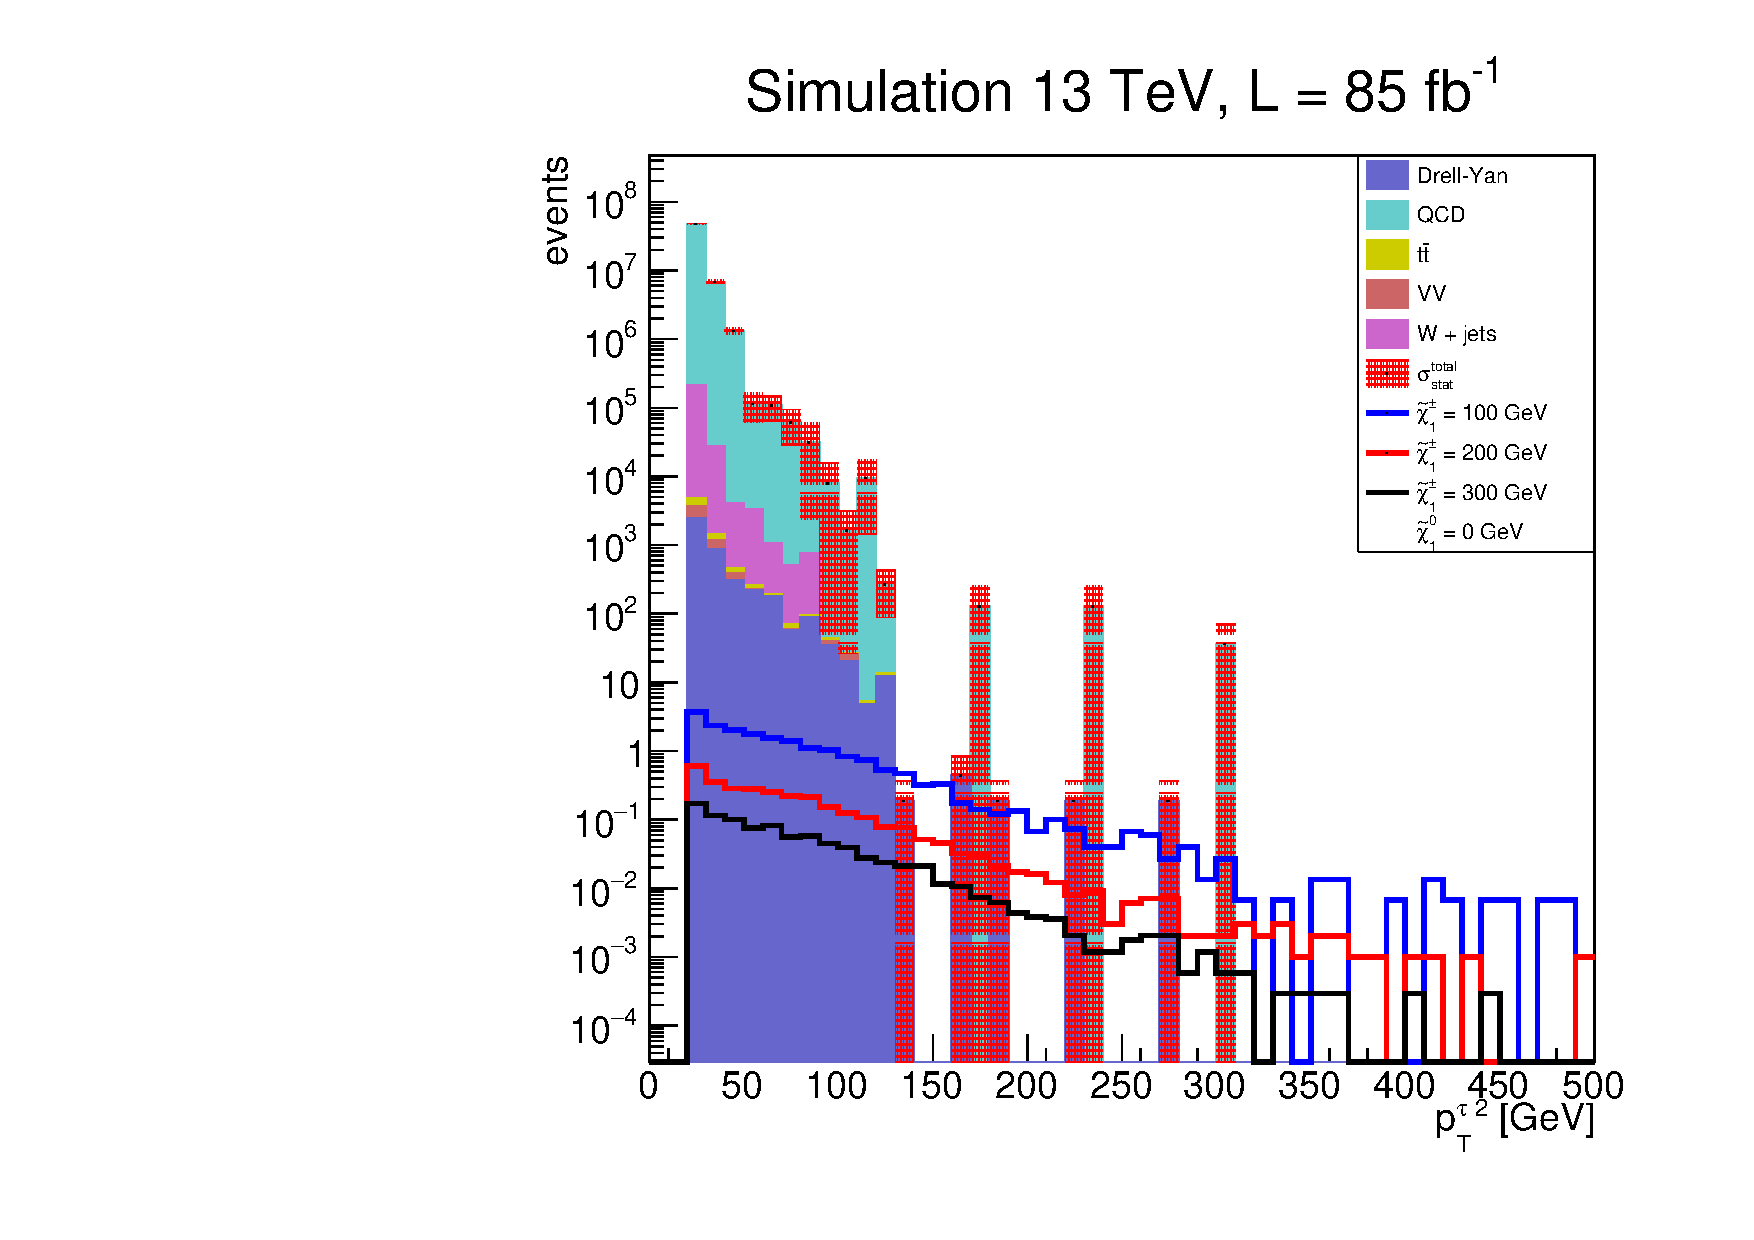
\includegraphics[width=0.5\textwidth]{analysis/pics/h_tau2pt_Tau2LooseIsoInclusiveVBFInverted.pdf}
	\end{tabular}
	\caption{(Left) Leading jet \pt distribution and (Right) and second leading \hadtau \pt distribution of selected signal and all MC background samples in control region 4.}
	\label{fig::crplots2_Tau2LooseIsoInclusiveVBFInverted_13tev}
\end{figure}

\clearpage

\section{Signal cross-section limits at 13 TeV}
\label{sec::xseclim_results}

This section shows the final results for the sensitivity study done on 13\tev simulated samples as function of the invariant mass of the di-jet candidate,  \met and the reconstructed \hadtau \pt. The different benchmark points were choses in term of different theoretical assumptions (fixed- and average-\stau-mass) and scenarios (uncompressed mass and compressed mass spectrum) for \charginopm and \neutralinoone masses of 100, 200, 300 400 and 500\gev. Given the trivial assumption that the cross section limit is strictly correlated to the reconstructed \hadtau \pt all the below results are shown considering a cut of 20\gev over this variable.

\todo{explain the table content, the limit plot and the cross section limit comparison}

\subsection*{Uncompressed scenario, fixed-\stau mass}

\FloatBarrier


\begin{figure}[tbh!]
	\centering
	\begin{tabular}{cc}
		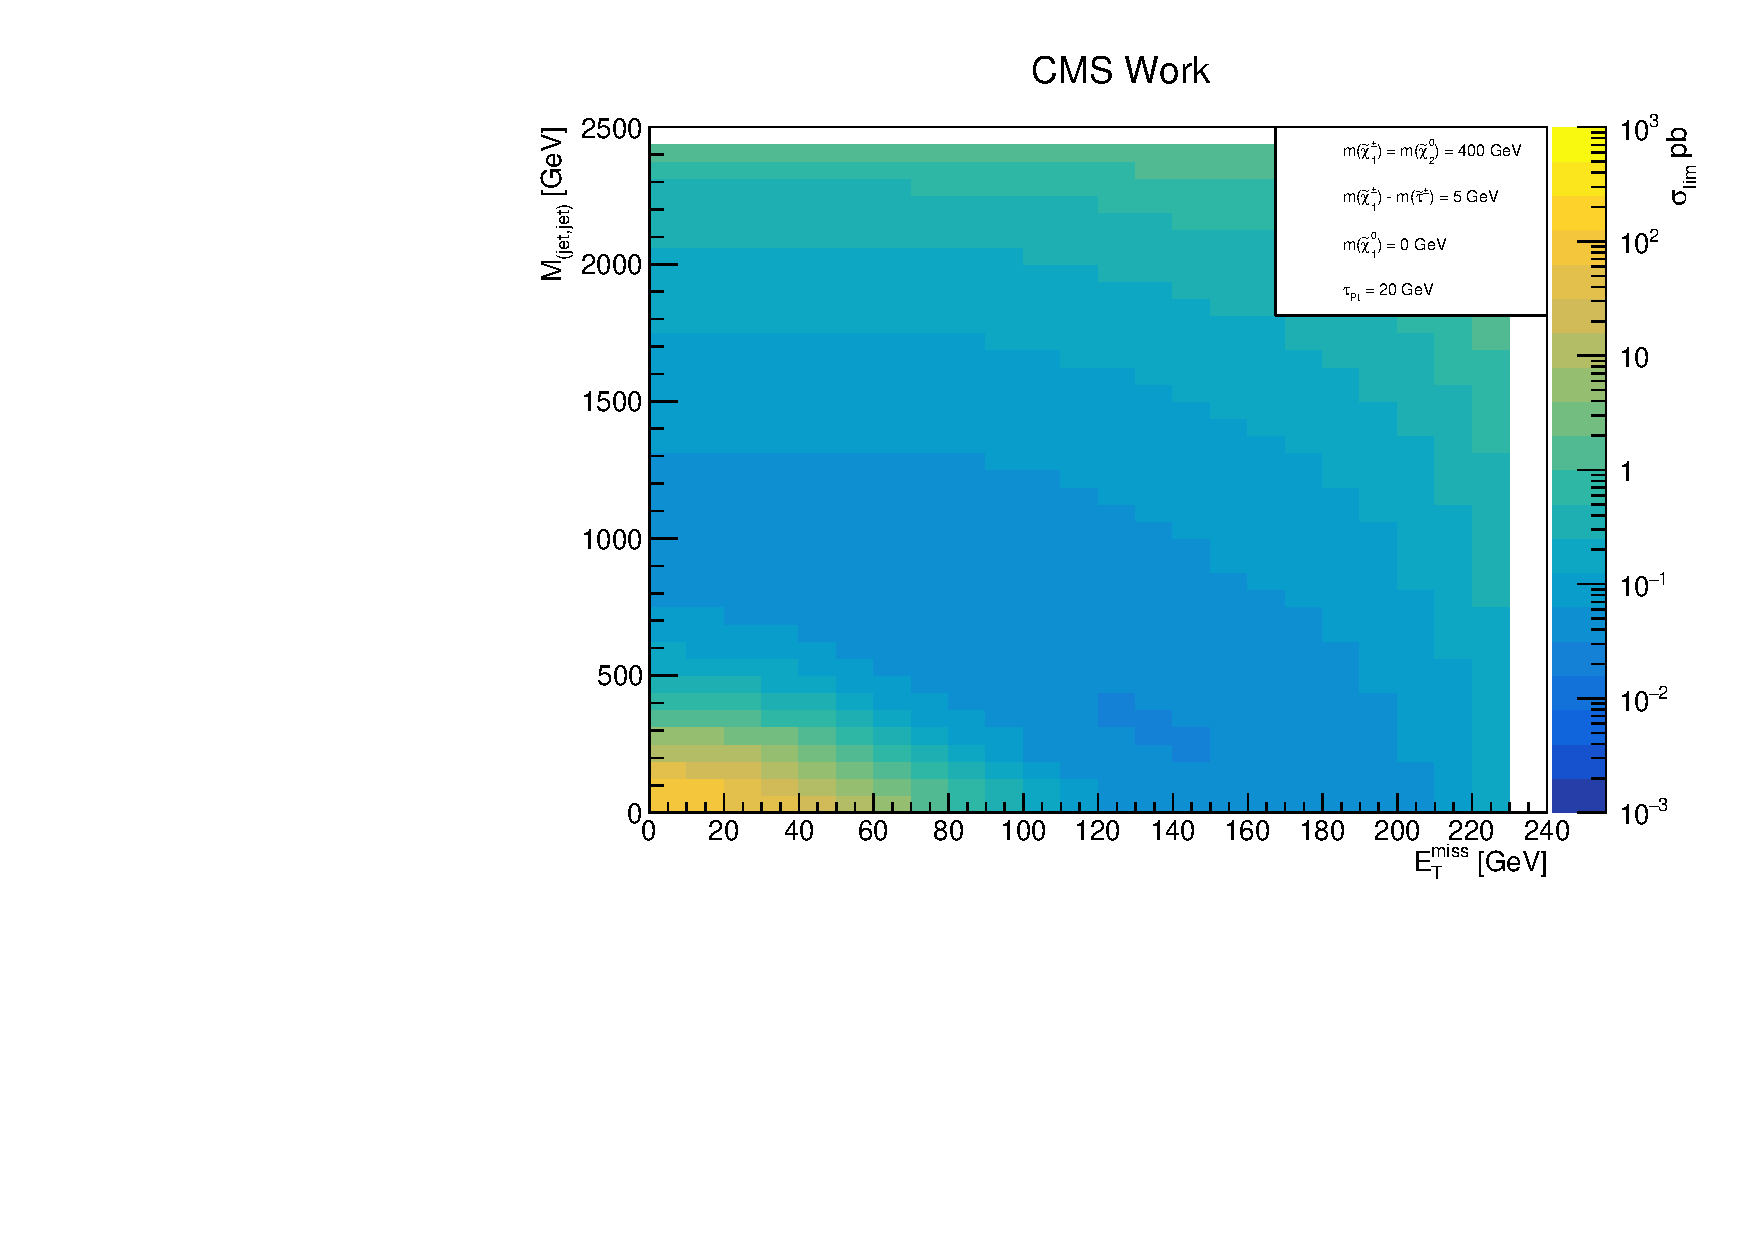
\includegraphics[width=0.75\textwidth]{analysis/pics/JetInvMass_vs_MET_xseclim_Chargino400_Stau395_LSP000_taupt20.pdf}
	\end{tabular}
	\caption{Cross section limit as function of $m_{jj}$ and \met for m(\charginopm) = m(\neutralinotwo) = 400 GeV,  m(\stau) = 395 GeV, and m(\neutralinoone) = 0 GeV and an offline selection on $\pt(\hadtau) <  20\gev$.}
	\label{fig::JetInvMass_vs_MET_xseclim_Chargino400_Stau395_LSP000_taupt20}
\end{figure}

\begin{table}
	\begin{center}
		
		\begin{tabular}{| c | c | c | c | }
			\toprule
			\multicolumn{4}{| c | }{m(\charginopm) = m(\stau) = 5\gev; m(\neutralinoone) = 0\gev} \\
			\midrule
			$\sigma_{lim}^{min}\pm(stat.)\pm(MC syst.)\pm(VBF syst.)$ [pb]  & m(\charginopm) = m(\neutralinotwo) [GeV] & \mjj [GeV] & \met [GeV] \\
			\midrule
			$0.033\pm0.002^{+0.003 + 0.001}_{-0.004-0.001}$ & $<$ 100 & $<$ 250  & $<$ 130 \\ 
			$0.033\pm0.002^{+0.003 + 0.001}_{-0.004-0.001}$ & $<$ 200 & $<$ 250  & $<$ 130 \\ 
			$0.034\pm0.002^{+0.003 + 0.001}_{-0.004-0.001}$ & $<$ 300 & $<$ 312.5  & $<$ 120 \\ 
			$0.030\pm0.001^{+0.002 + 0.001}_{-0.003-0.000}$ & $<$ 400 & $<$ 312.5  & $<$ 130 \\ 
			$0.030\pm0.001^{+0.003+ 0.001}_{-0.003-0.000}$ & $<$ 500 & $<$ 250  & $<$ 130 \\ 
			\bottomrule
		\end{tabular}\caption{Cross section limit minimum reached at the given cuts for $m_{jj}$, \met and an increasing \charginopm = \neutralinotwo for the uncompressed mass spectra and fixed-\stau mass  benchmark point.}
		\label{table::xseclim_uncompressed_fixedmass}
	\end{center}
\end{table}

\begin{figure}[tbh!]
	\centering
	\begin{tabular}{cc}
		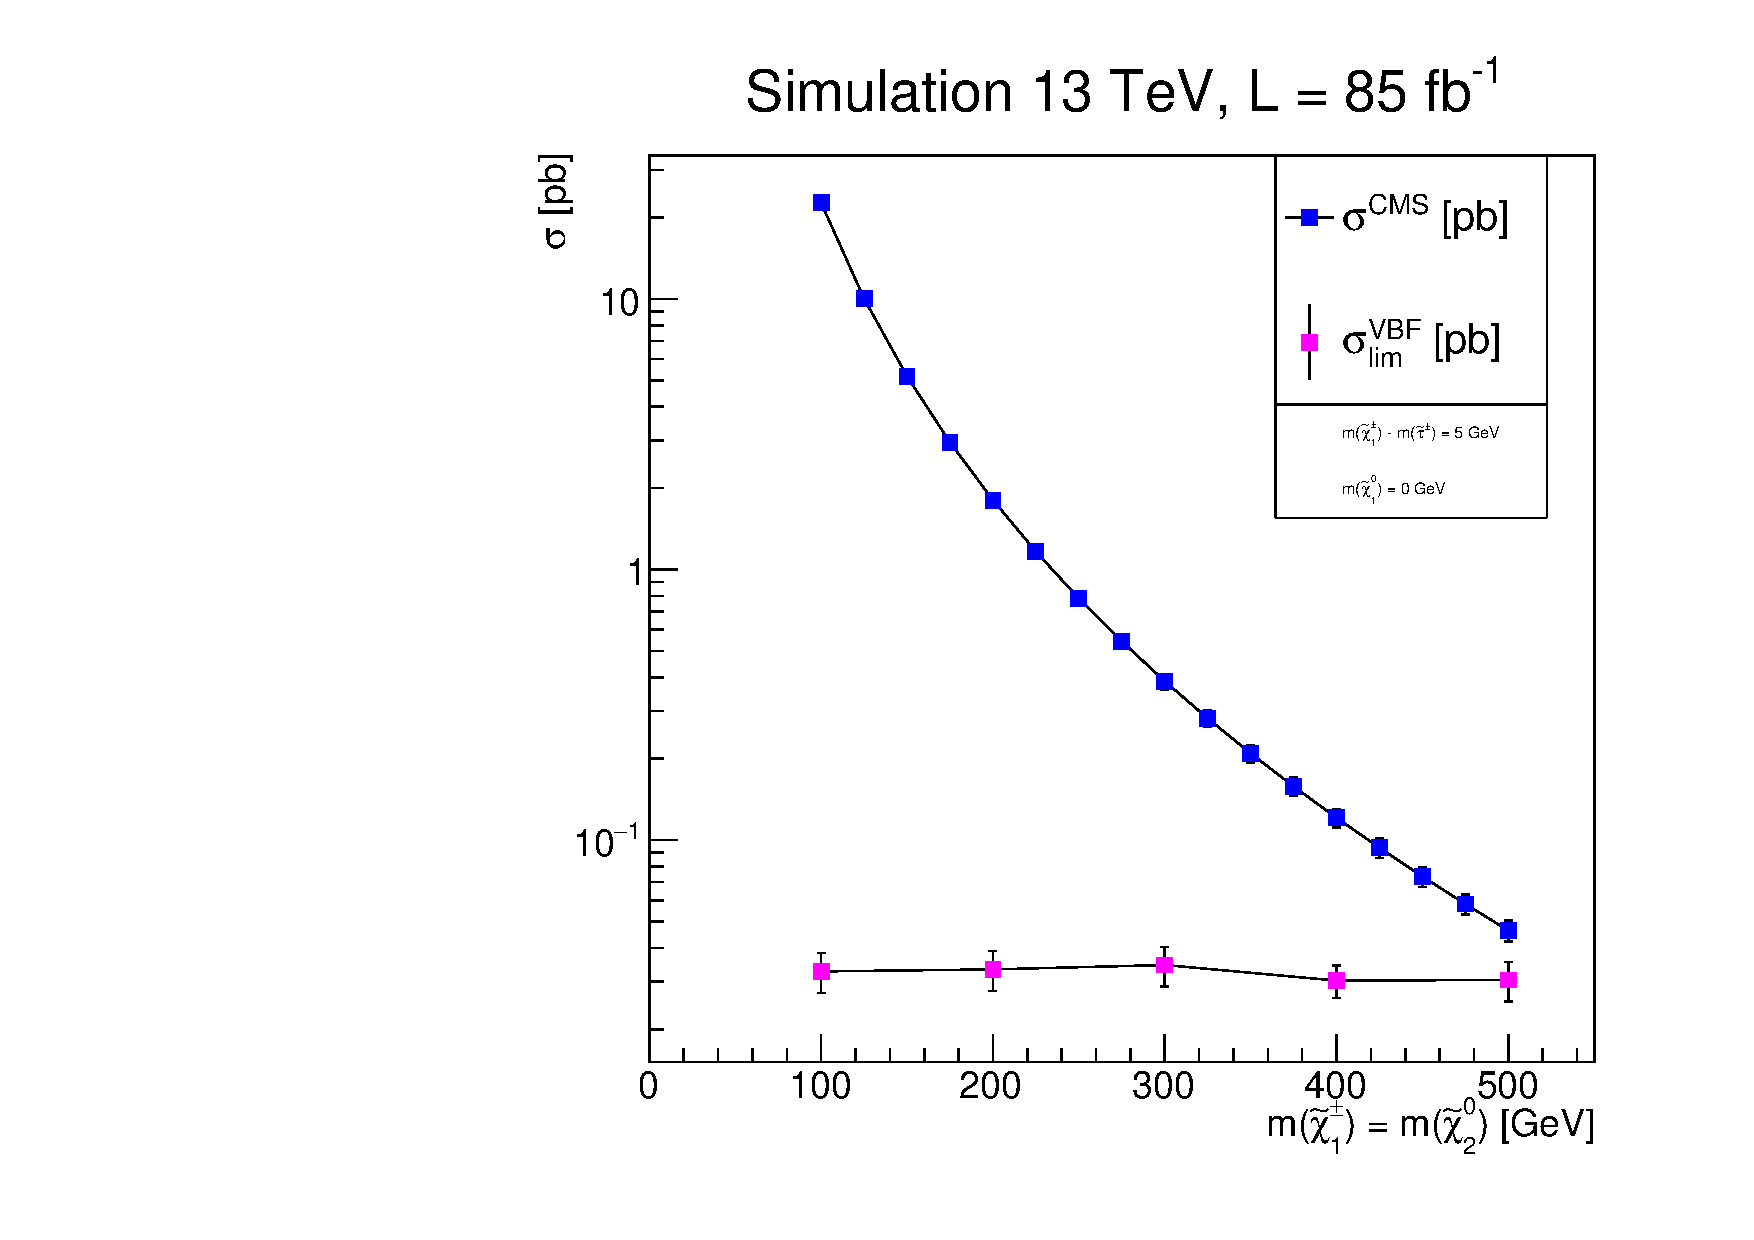
\includegraphics[width=0.75\textwidth]{analysis/pics/out_xsecmin_lsp000_stauclose.pdf}
	\end{tabular}
	\caption{Comparison between the cross section limit taken from the study over the uncompressed mass spectra and fixed-\stau mass benchmark point and the official CMS cross sections calculated using the \texttt{resummino} code from B. Fuks et al with CTEQ6.6 and MSTW2008nlo90cl PDFs \cite{Fuks:2013vua}.}
	\label{fig::out_xsecmin_lsp000_stauclose}
\end{figure}


\FloatBarrier

\subsection*{Compressed scenario, fixed-\stau mass}


\begin{figure}[tbh!]
	\centering
	\begin{tabular}{cc}
		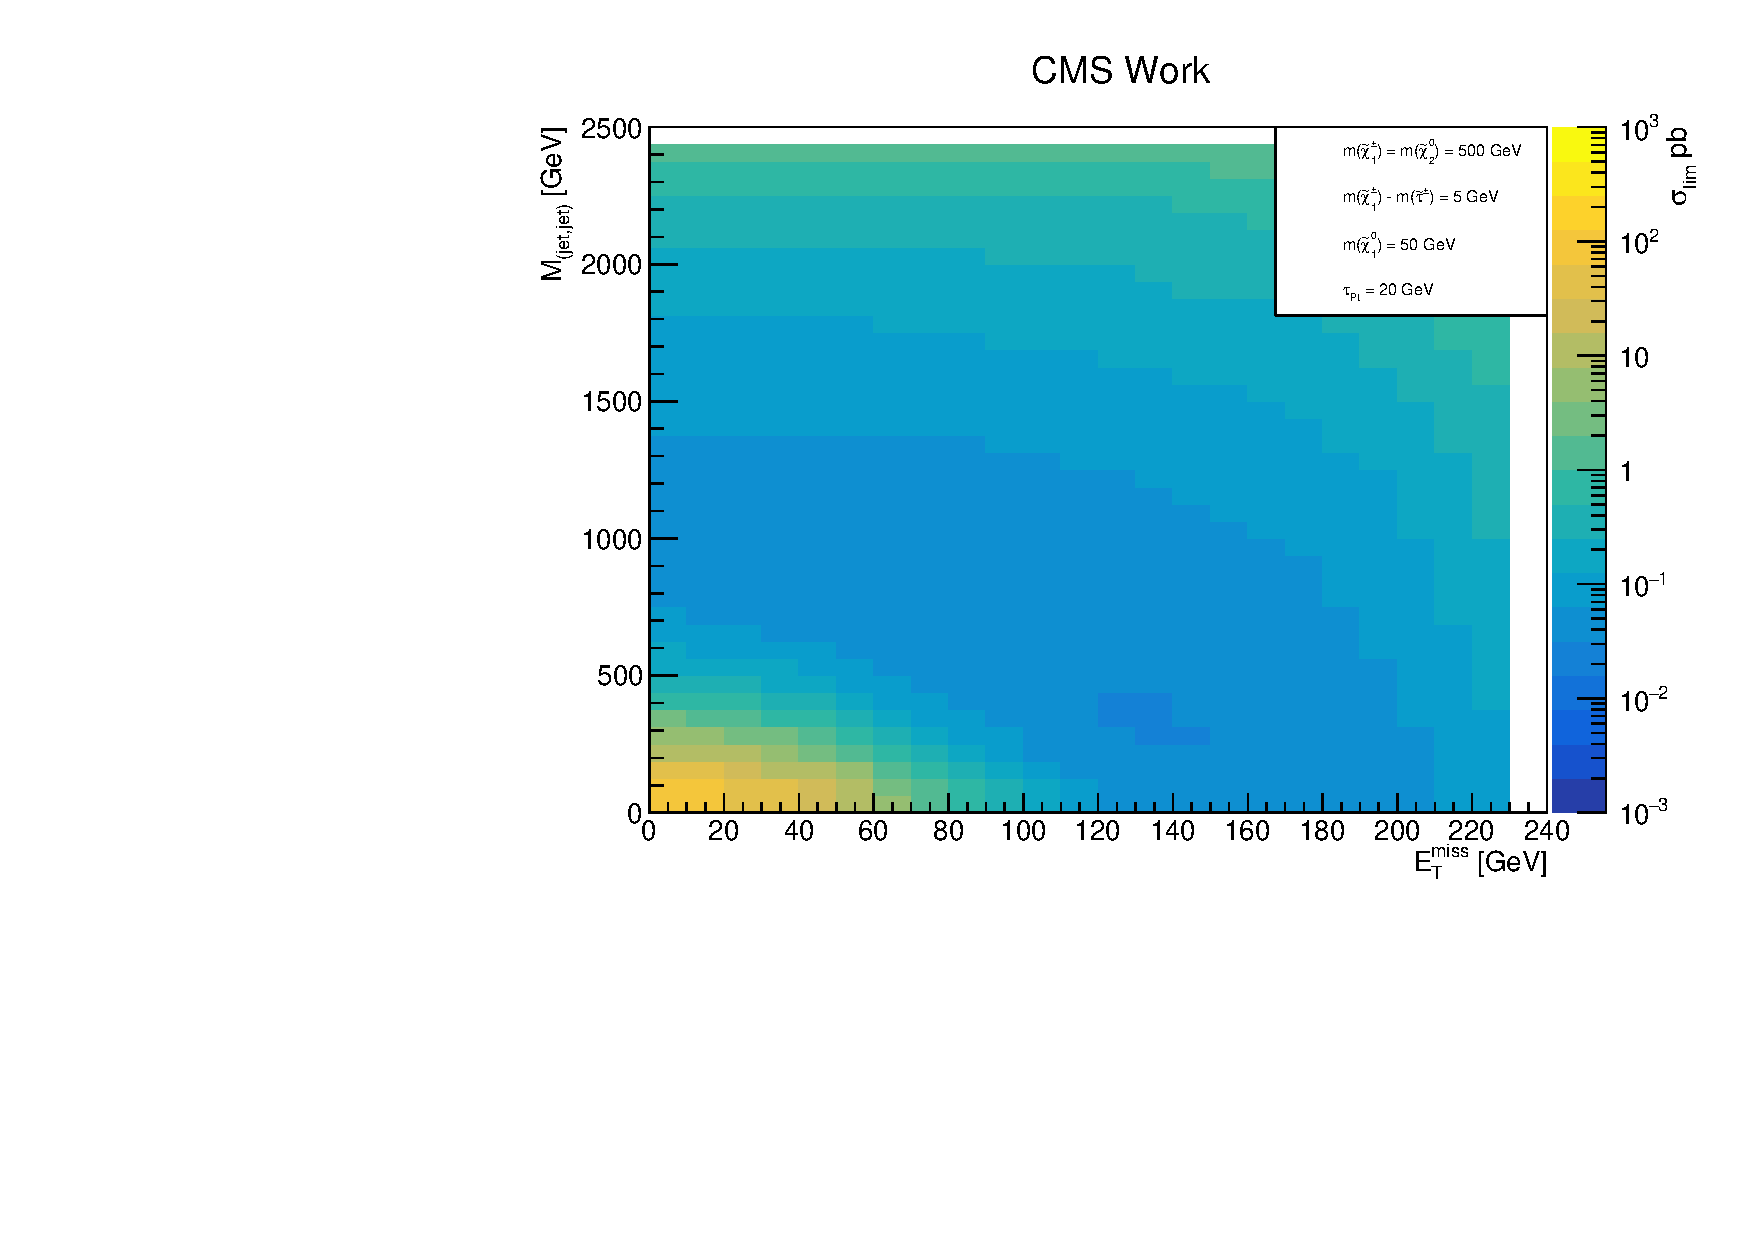
\includegraphics[width=0.75\textwidth]{analysis/pics/JetInvMass_vs_MET_xseclim_Chargino500_Stau495_LSP050_taupt20.pdf}
	\end{tabular}
	\caption{Cross section limit as function of $m_{jj}$ and \met for m(\charginopm) = m(\neutralinotwo) = 500 GeV,  m(\stau) = 495 GeV, and m(\neutralinoone) = 50 GeV and an offline selection on $\pt(\hadtau) <  20\gev$.}
	\label{fig::JetInvMass_vs_MET_xseclim_Chargino500_Stau495_LSP050_taupt20}
\end{figure}

\begin{table}
	\begin{center}
		
		\begin{tabular}{| c | c | c | c | }
			\toprule
			\multicolumn{4}{| c | }{m(\charginopm) = m(\stau) = 5\gev; m(\charginopm) - m(\neutralinoone) = 50\gev} \\
			\midrule
			$\sigma_{lim}^{min}\pm(stat.)\pm(MC syst.)\pm(VBF syst.)$ [pb]  & m(\charginopm) = m(\neutralinotwo) [GeV] & \mjj [GeV] & \met [GeV] \\
			\midrule
			$0.033\pm0.002^{+0.003 + 0.001}_{-0.004-0.001}$ & $<$ 100 & $<$ 250  & $<$ 130 \\ 
			$0.033\pm0.002^{+0.003 + 0.001}_{-0.004-0.001}$ & $<$ 200 & $<$ 312.5  & $<$ 120 \\ 
			$0.033\pm0.001^{+0.002 + 0.001}_{-0.003-0.000}$ & $<$ 300 & $<$ 312.5  & $<$ 130 \\ 
			$0.031\pm0.001^{+0.002 + 0.001}_{-0.003-0.001}$ & $<$ 400 & $<$ 250  & $<$ 130 \\ 
			$0.030\pm0.001^{+0.002 + 0.001}_{-0.003-0.000}$ & $<$ 500 & $<$ 312.5  & $<$ 130 \\ 
			\bottomrule
		\end{tabular}\caption{Cross section limit minimum reached at the given cuts for $m_{jj}$, \met and an increasing \charginopm = \neutralinotwo for the compressed mass spectra and fixed-\stau mass  benchmark point.}
		\label{table::xseclim_compressed_fixedmass}
	\end{center}
\end{table}

\begin{figure}[tbh!]
	\centering
	\begin{tabular}{cc}
		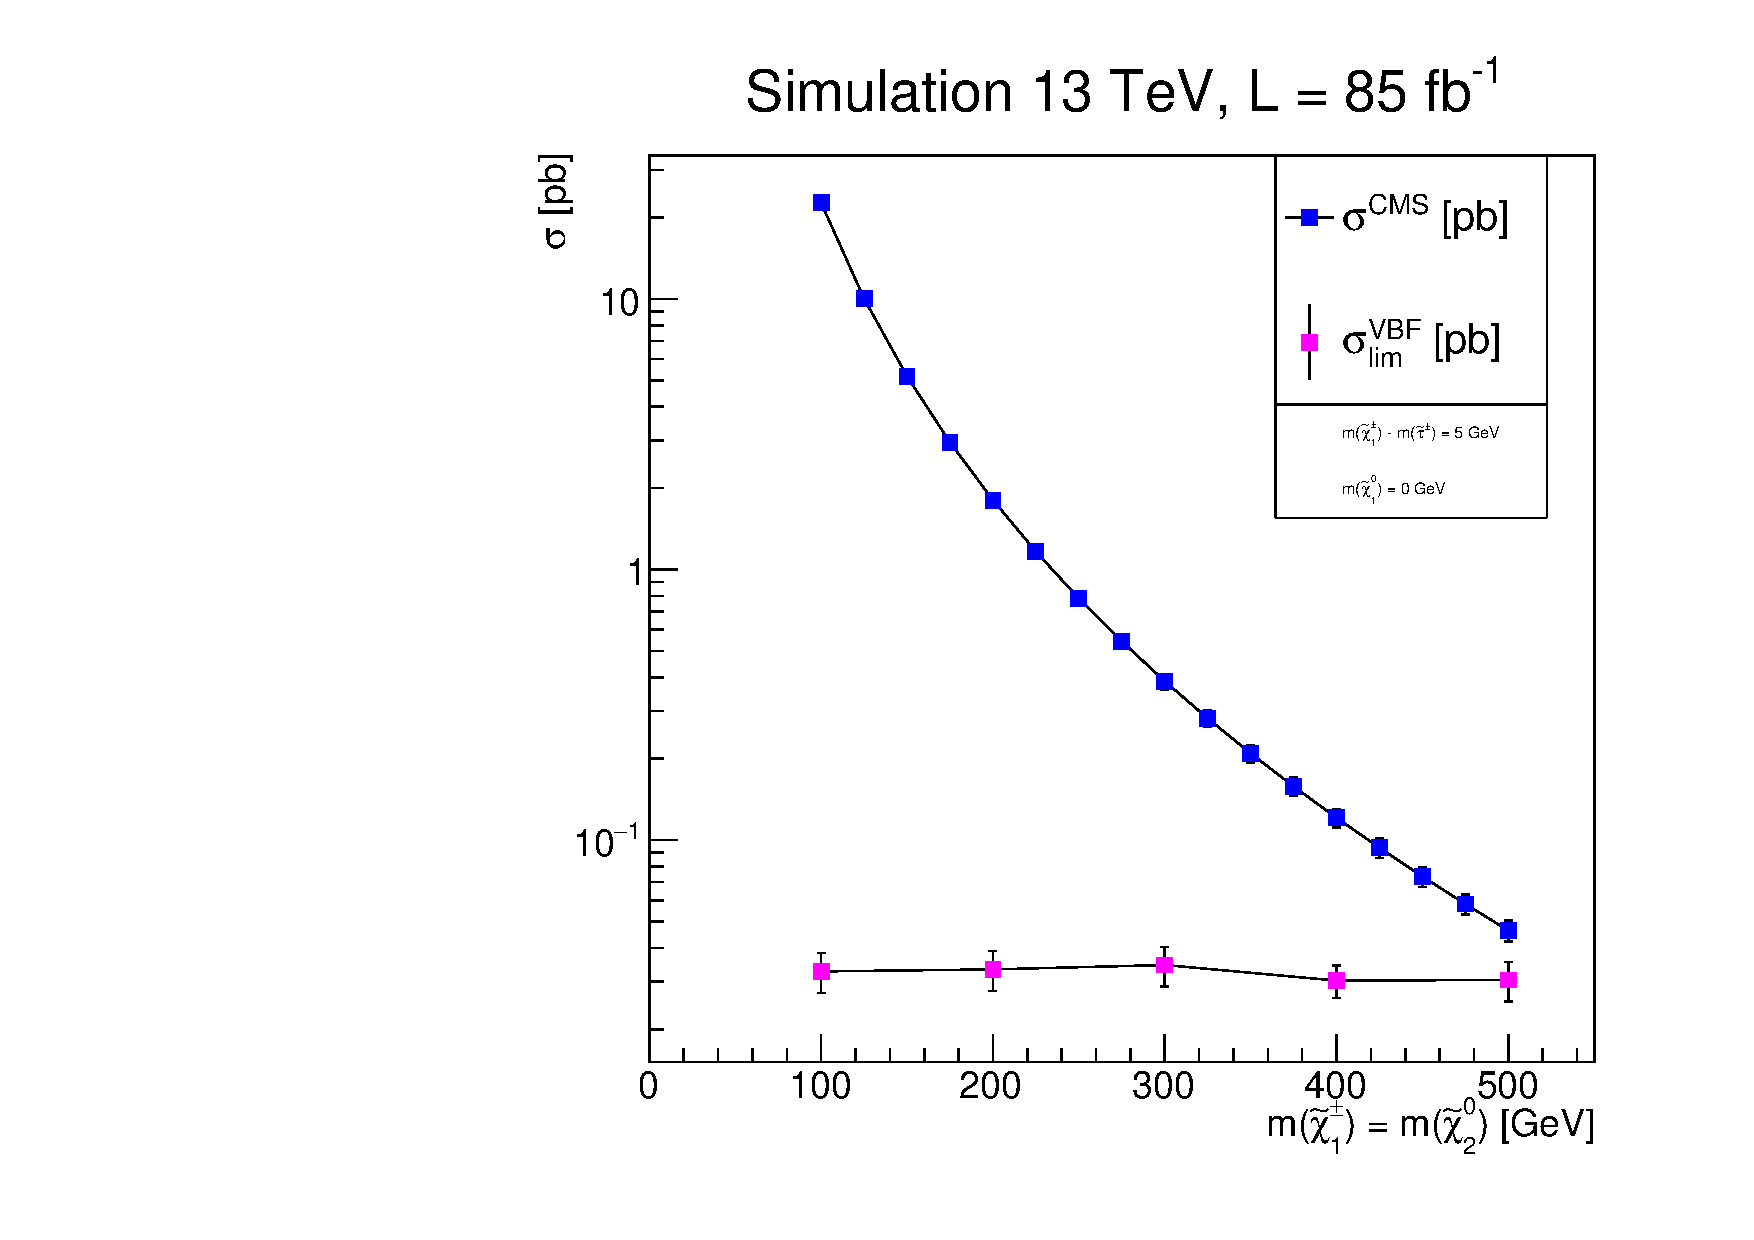
\includegraphics[width=0.75\textwidth]{analysis/pics/out_xsecmin_lsp000_stauclose.pdf}
	\end{tabular}
	\caption{Comparison between the cross section limit taken from the study over the compressed mass spectra and fixed-\stau mass benchmark point and the official CMS cross sections calculated using the \texttt{resummino} code from B. Fuks et al with CTEQ6.6 and MSTW2008nlo90cl PDFs \cite{Fuks:2013vua}.}
	\label{fig::out_xsecmin_lsp050_stauclose}
\end{figure}


\FloatBarrier

\subsection*{Uncompressed scenario, average-\stau mass}


\begin{figure}[tbh!]
	\centering
	\begin{tabular}{cc}
		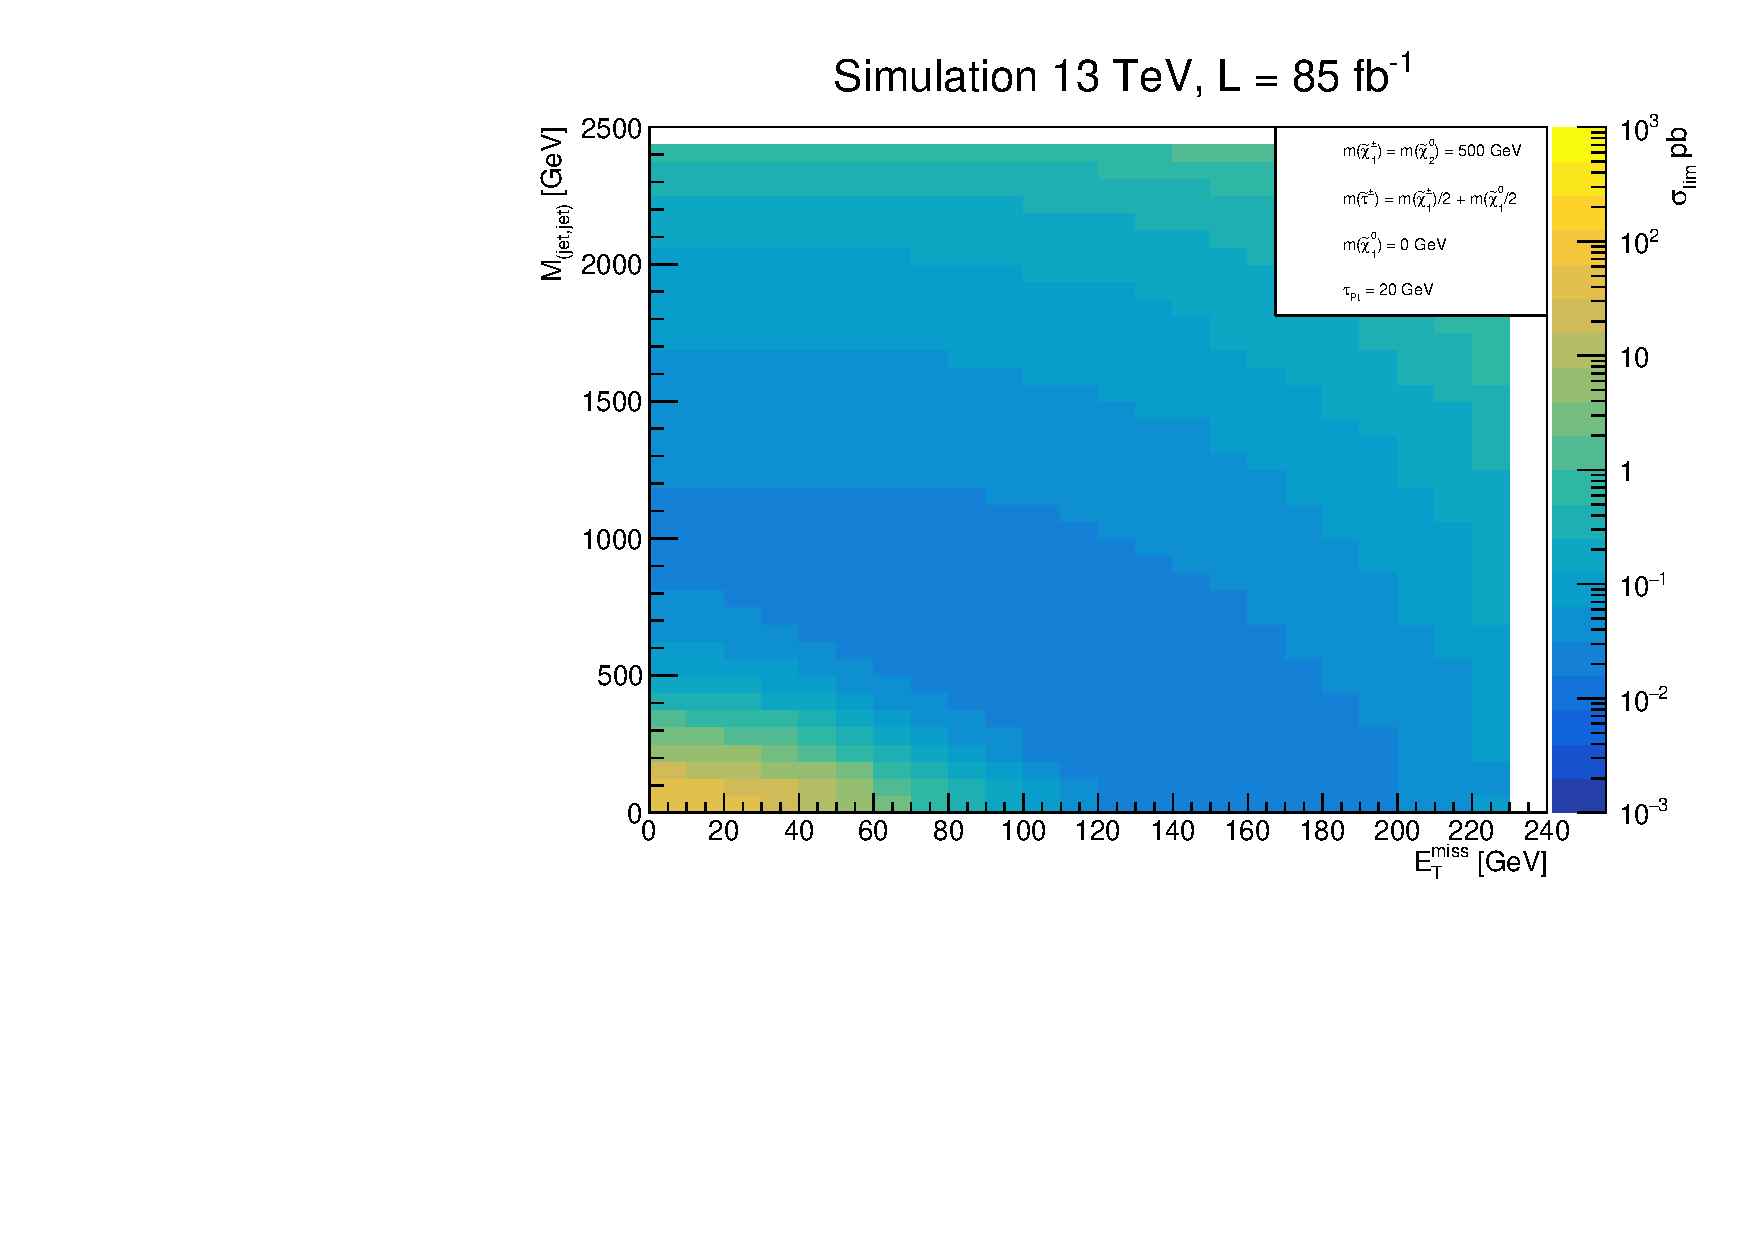
\includegraphics[width=0.75\textwidth]{analysis/pics/JetInvMass_vs_MET_xseclim_Chargino500_Stau250_LSP000_taupt20.pdf}
	\end{tabular}
	\caption{Cross section limit as function of $m_{jj}$ and \met for m(\charginopm) = m(\neutralinotwo) = 500 GeV,  m(\stau) = 250 GeV, and m(\neutralinoone) = 0 GeV and an offline selection on $\pt(\hadtau) <  20\gev$.}
	\label{fig::JetInvMass_vs_MET_xseclim_Chargino500_Stau250_LSP000_taupt20}
\end{figure}

\begin{table}
	\begin{center}
		
		\begin{tabular}{| c | c | c | c | }
			\toprule
			\multicolumn{4}{| c | }{m(\stau) = 0.5 m(\neutralinoone) + 0.5 m(\charginopm) ; m(\neutralinoone) = 0\gev} \\
			\midrule
			$\sigma_{lim}^{min}\pm(stat.)\pm(MC syst.)\pm(VBF syst.)$ [pb]  & m(\charginopm) = m(\neutralinotwo) [GeV] & \mjj [GeV] & \met [GeV] \\
			\midrule
				$0.083\pm0.005^{+0.007 + 0.003}_{-0.009-0.001}$ & $<$ 100 & $<$ 312.5  & $<$ 120 \\ 
				$0.036\pm0.002^{+0.003 + 0.001}_{-0.004-0.001}$ & $<$ 200 & $<$ 375  & $<$ 110 \\ 
				$0.024\pm0.001^{+0.002 + 0.001}_{-0.003-0.000}$ & $<$ 300 & $<$ 250  & $<$ 130 \\ 
				$0.019\pm0.001^{+0.002 + 0.001}_{-0.002-0.000}$ & $<$ 400 & $<$ 250  & $<$ 130 \\ 
				$0.017\pm0.001^{+0.002 + 0.001}_{-0.002-0.000}$ & $<$ 500 & $<$ 250  & $<$ 130 \\ 
			\bottomrule
		\end{tabular}\caption{Cross section limit minimum reached at the given cuts for $m_{jj}$, \met and an increasing \charginopm = \neutralinotwo for the uncompressed mass spectra and average-\stau mass benchmark point.}
		\label{table::xseclim_uncompressed_averagemass}
	\end{center}
\end{table}

\begin{figure}[tbh!]
	\centering
	\begin{tabular}{cc}
		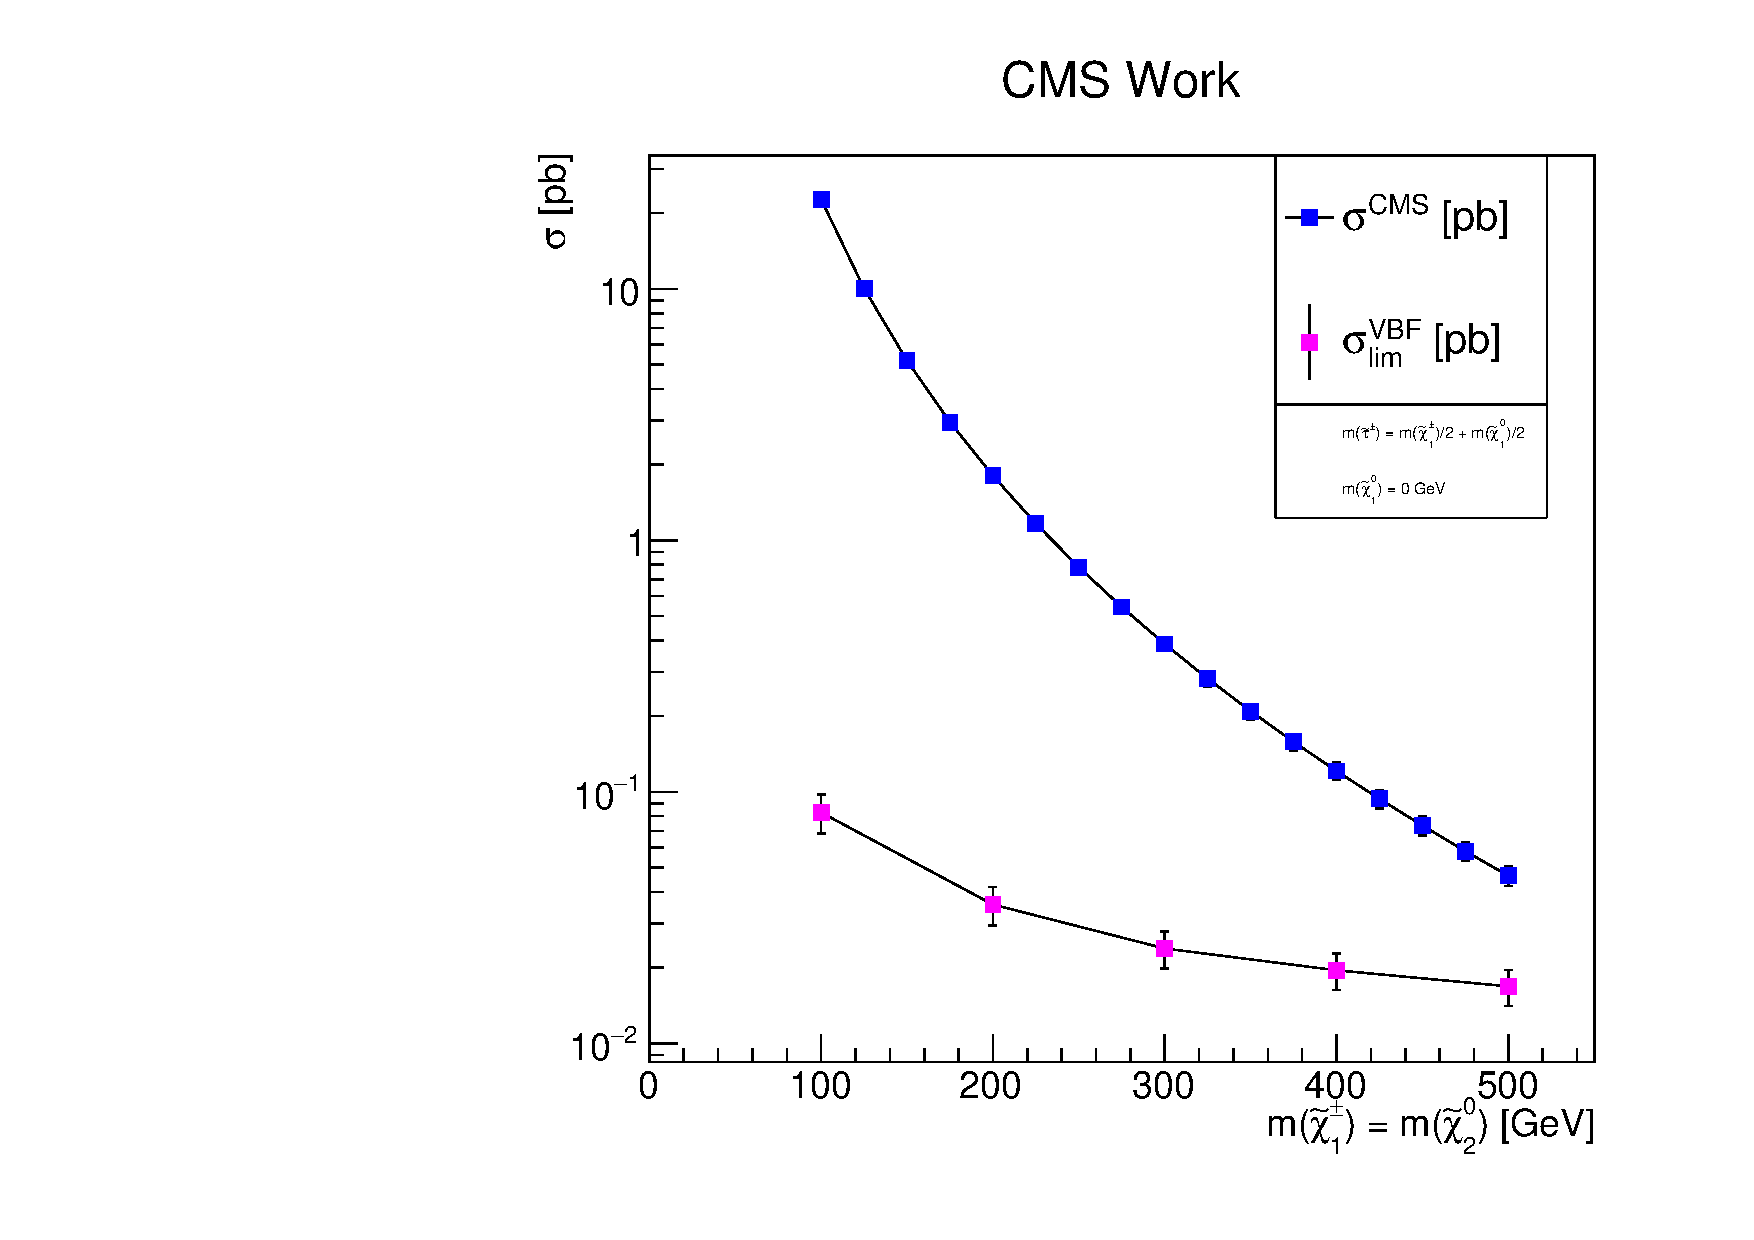
\includegraphics[width=0.75\textwidth]{analysis/pics/out_xsecmin_lsp000_staufar.pdf}
	\end{tabular}
	\caption{Comparison between the cross section limit taken from the study over the uncompressed mass spectra and average-\stau mass benchmark point and the official CMS cross sections calculated using the \texttt{resummino} code from B. Fuks et al with CTEQ6.6 and MSTW2008nlo90cl PDFs \cite{Fuks:2013vua}.}
	\label{fig::out_xsecmin_lsp000_staufar}
\end{figure}

\FloatBarrier

\subsection*{Compressed scenario, average-\stau mass}


\begin{figure}[tbh!]
	\centering
	\begin{tabular}{cc}
		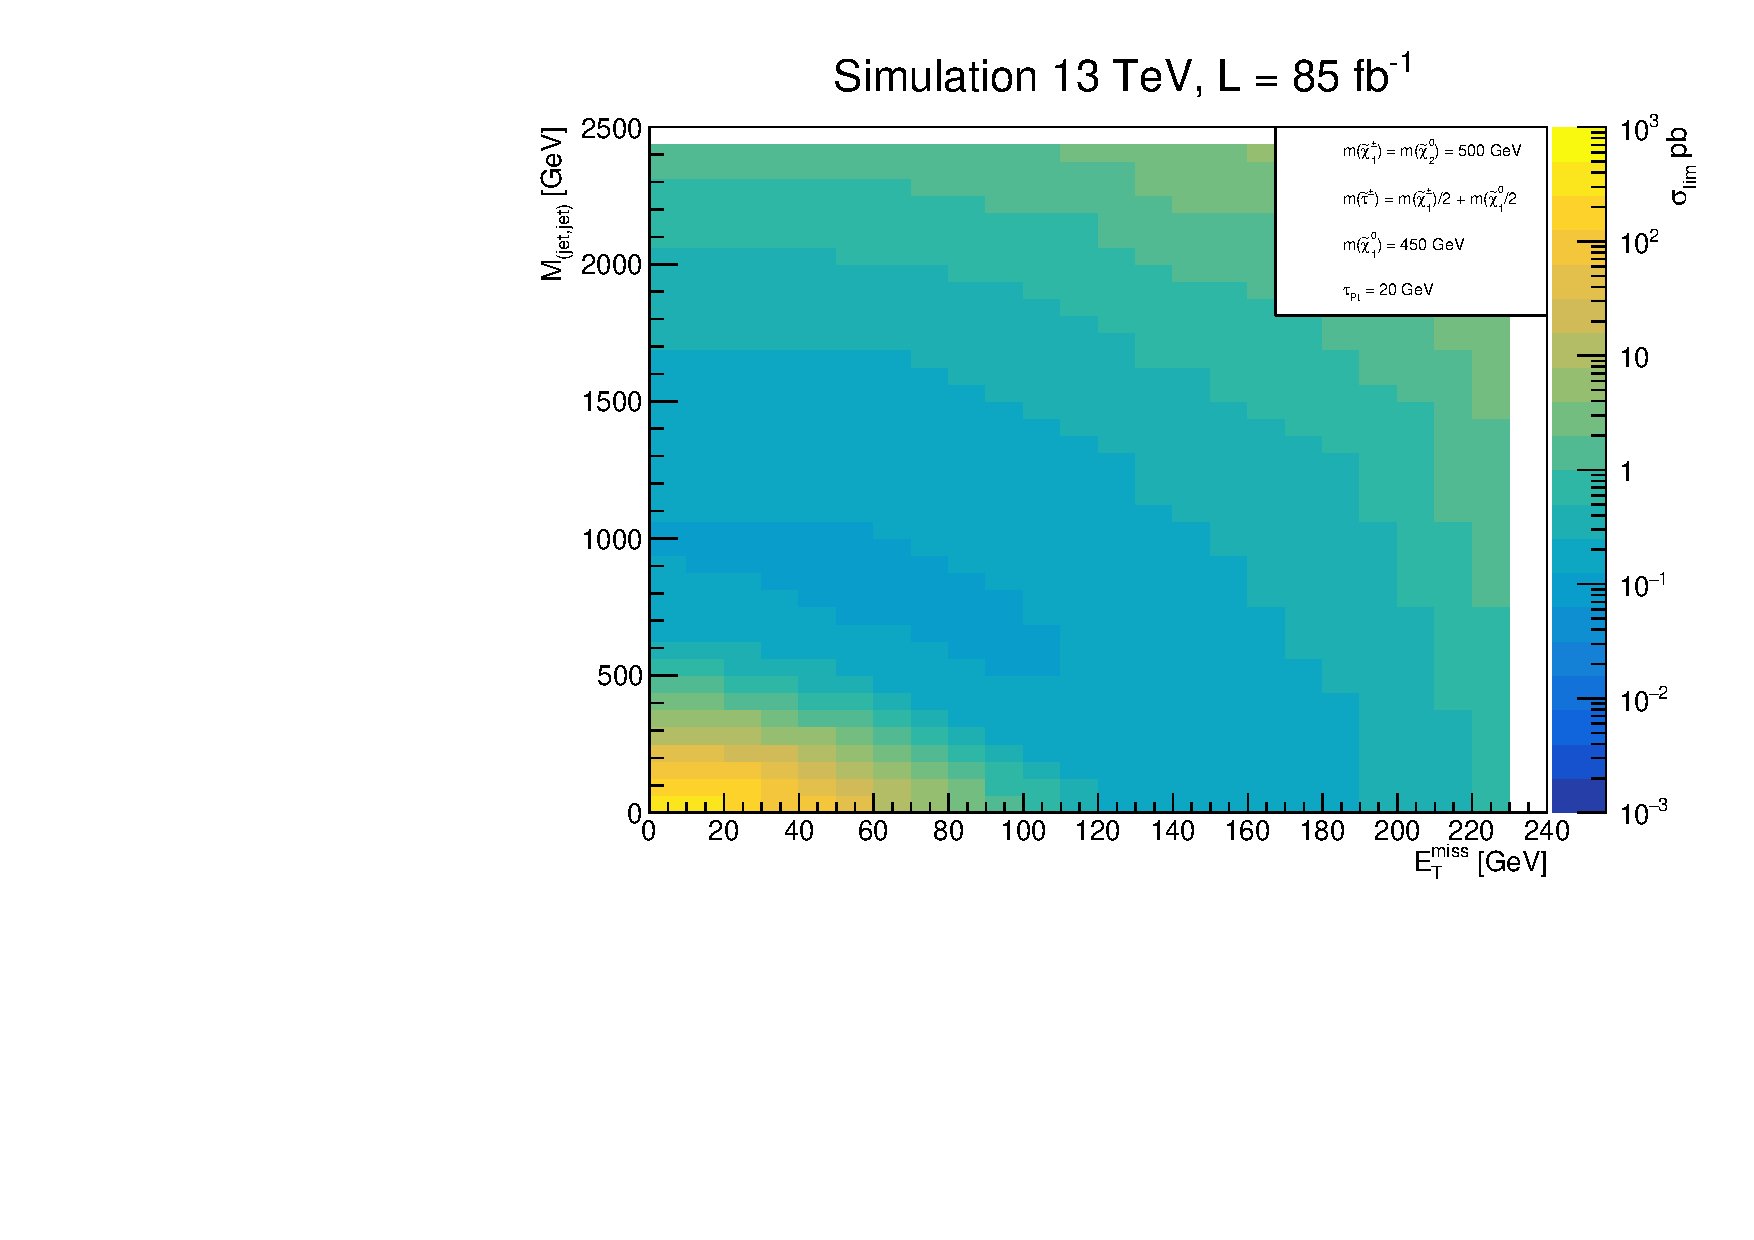
\includegraphics[width=0.75\textwidth]{analysis/pics/JetInvMass_vs_MET_xseclim_Chargino500_Stau475_LSP450_taupt20.pdf}
	\end{tabular}
	\caption{Cross section limit as function of $m_{jj}$ and \met for m(\charginopm) = m(\neutralinotwo) = 500 GeV,  m(\stau) = 475 GeV, and m(\neutralinoone) = 450 GeV and an offline selection on $\pt(\hadtau) <  20\gev$.}
	\label{fig::JetInvMass_vs_MET_xseclim_Chargino500_Stau475_LSP450_taupt20}
\end{figure}

\begin{table}
	\begin{center}
		
		\begin{tabular}{| c | c | c | c | }
			\toprule
			\multicolumn{4}{| c | }{m(\stau) = 0.5 m(\neutralinoone) + 0.5 m(\charginopm) ; m(\charginopm) - m(\neutralinoone) = 50\gev} \\
			\midrule
			$\sigma_{lim}^{min}\pm(stat.)\pm(MC syst.)\pm(VBF syst.)$ [pb]  & m(\charginopm) = m(\neutralinotwo) [GeV] & \mjj [GeV] & \met [GeV] \\
			\midrule
				$0.153\pm0.011^{+0.012 + 0.005}_{-0.014-0.002}$ & $<$ 100 & $<$ 500  & $<$ 100 \\ 
				$0.148\pm0.011^{+0.014 + 0.005}_{-0.017-0.002}$ & $<$ 200 & $<$ 375  & $<$ 110 \\ 
				$0.157\pm0.011^{+0.013 + 0.005}_{-0.015-0.002}$ & $<$ 300 & $<$ 562.5  & $<$ 90 \\ 
				$0.150\pm0.011^{+0.014 + 0.005}_{-0.016-0.002}$ & $<$ 400 & $<$ 312.5  & $<$ 120 \\ 
				$0.115\pm0.007^{+0.010 + 0.004}_{-0.012-0.002}$ & $<$ 500 & $<$ 750  & $<$ 60 \\
			\bottomrule
		\end{tabular}\caption{Cross section limit minimum reached at the given cuts for $m_{jj}$, \met and an increasing \charginopm = \neutralinotwo for the compressed mass spectra and average-\stau mass benchmark point.}
		\label{table::xseclim_compressed_averagemass}
	\end{center}
\end{table}

\begin{figure}[tbh!]
	\centering
	\begin{tabular}{cc}
		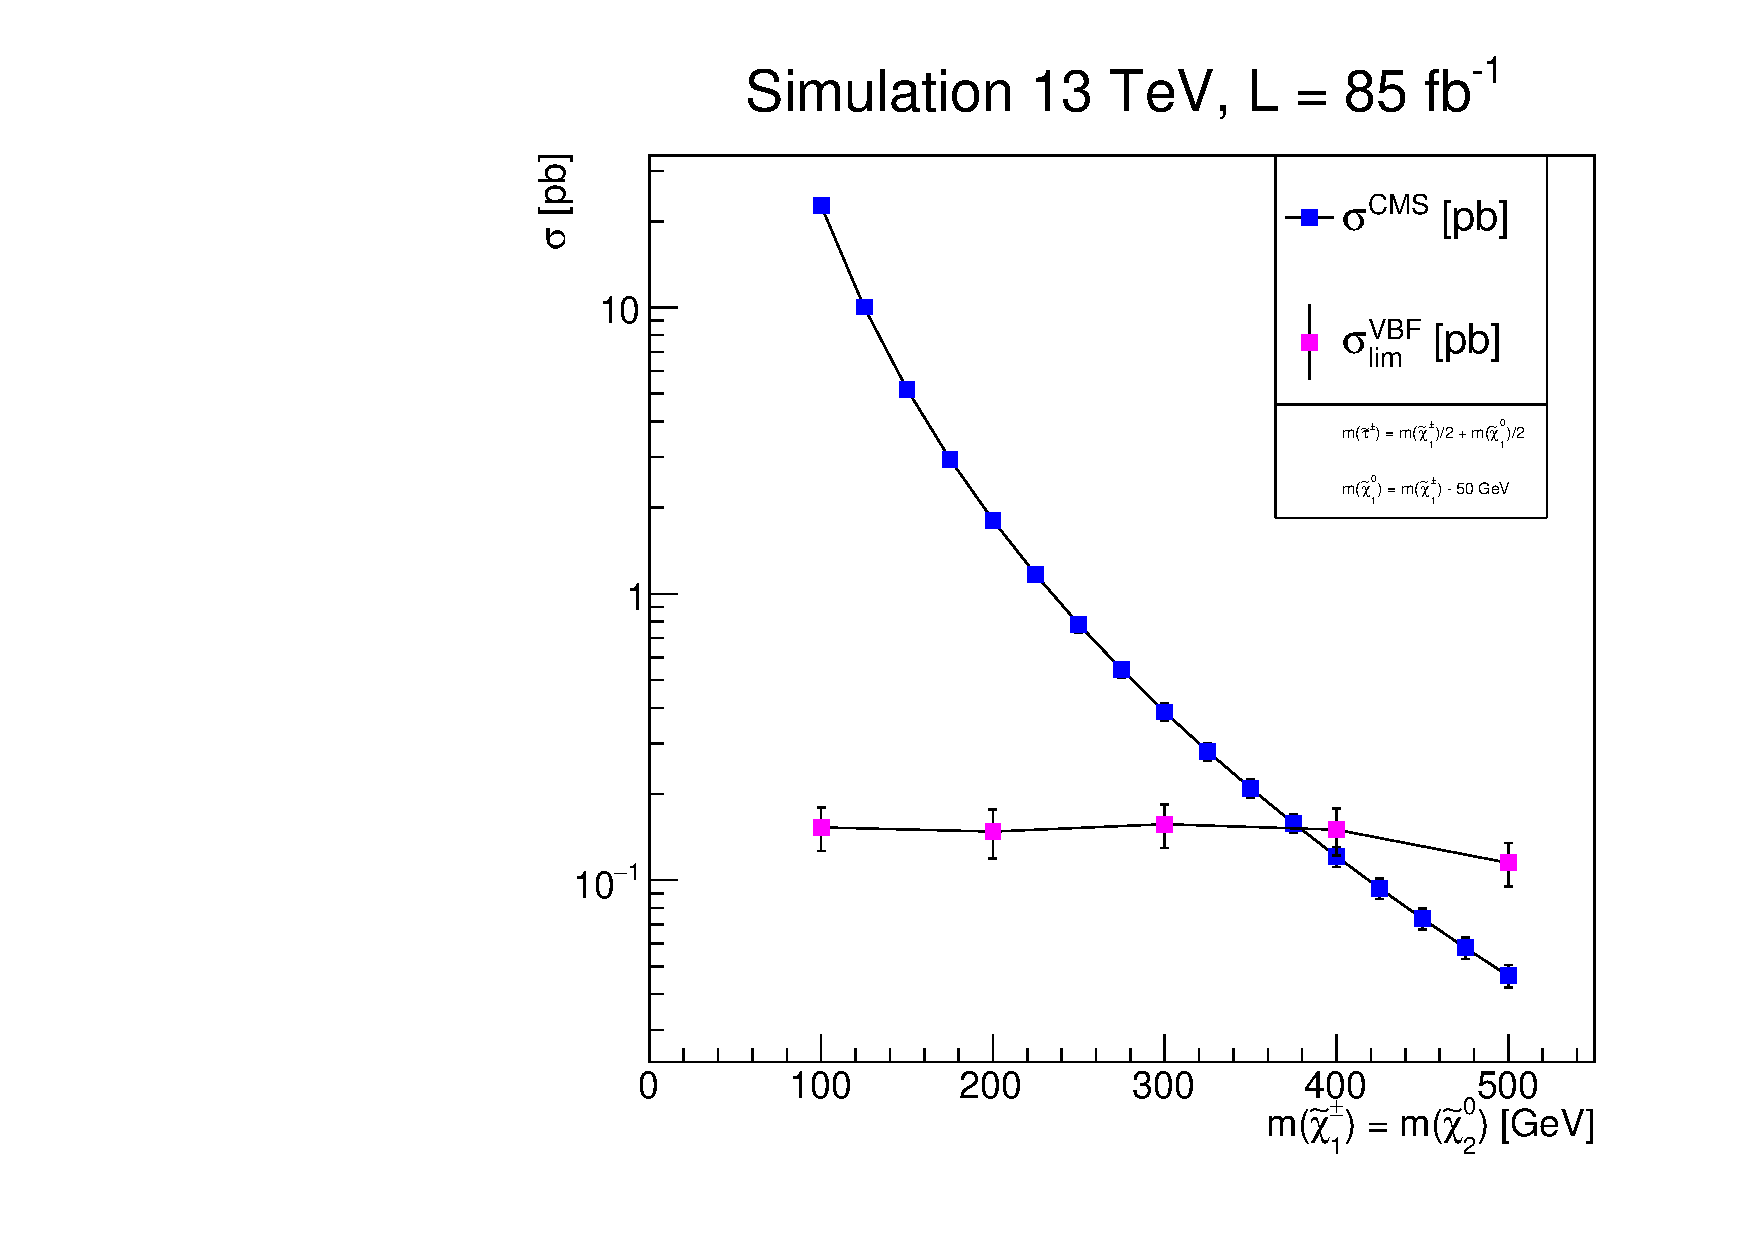
\includegraphics[width=0.75\textwidth]{analysis/pics/out_xsecmin_lspcomp_stauclose.pdf}
	\end{tabular}
	\caption{Comparison between the cross section limit taken from the study over the compressed mass spectra and average-\stau mass benchmark point and the official CMS cross sections calculated using the \texttt{resummino} code from B. Fuks et al with CTEQ6.6 and MSTW2008nlo90cl PDFs \cite{Fuks:2013vua}.}
	\label{fig::out_xsecmin_lspcomp_stauclose}
\end{figure}

\FloatBarrier

